\chapter{First Order Models}

\section{Birth, Death, and Immigration Exploration}
\subsection*{Supplies}
1 partner, 1 cup, 1 handfull or bag of M\&M's, and 1 computer with access to Moodle and
Excel.
\subsection*{Scenarios}
The M\&M's in this activity represent a very fragile species with a high death rate.  To
determine which M\&M's survive and which die in a given year we will shake the M\&M's and
pour them on the table.  The M\&M's that land with the M up unfortunately die.  The
remaining M\&M's survive for another year.
\begin{description}
    \item[Scenario \#1 (Deaths)] Count the number of M\&M's in your cup and track the
        number of M\&M's remaining  until the species goes extinct.  Add your data to the
        Google Sheet linked from Moodle.
    \item[Scenario \#2 (Deaths and Immigration):] In this scenario, every M\&M that lands
        M-up will die, but at the end of the year there are 5 new M\&M's added to the
        population due to immigration. Track the number of M\&M's remaining until you
        believe that the population has reached a steady state.  Add your data to the
        second tab of the Google Sheet linked from Moodle.
    \item[Scenario \#3 (Births, Deaths, and Immigration):] In this final scenario, every
        M\&M that lands M-up will die, and at the end of the year there are 5 new M\&M's
        added to the population due to immigration.  After the immigration occurs, 10\% of
        the remaining M\&M's give birth to new M\&M's.  Add these births to the
        population.  Track the number of M\&M's (after the death, immigration, and the
        births) until you think the population has reached a steady state.  input your
        data into the Google Sheet, and move to the next year.  
\end{description}

\subsection*{Mathematical Modeling}
Our goal is to find a function that models each scenario. Copy your data sets from the
Google Sheet to your own machines and try to determine the type of function that best
models this scenario.  When you write your functions, use the variable $n$ for the time.  

Remember, we are trying to find a mathematical function that best models the scenario.
That does not necessarily mean that you should be doing any data fitting!  
Instead, you should try two methods:
\begin{enumerate}
    \item Can you find an algebraic function that appears to fit your data?
        \[ M(n) = \underline{\hspace{2in}} \]
    \item Or, can you write an expression for
        how the population changes? In other words,
        \[ \text{number of \underline{new} M\&M's at year $n$} = \underline{\hspace{2in}} \]
\end{enumerate}


\newpage\section{Models for Death, Birth, and Immigration}
\begin{problem}
    In the death, birth, and immigration exploration you should have generated data with your
    class for the three scenarios. Go back to the Google Sheet with all of the data, copy
    your group's data to Excel and make the following plots:
    \begin{itemize}
        \item A plot with population on the horizontal axis and average rate of change of the
            population for the death model on the vertical axis.  You will need to
            calculate the average rate of change in Excel first.
        \item A plot with population on the horizontal axis and average rate of change of the
            population for the death \& immigration model on the vertical axis.  You will need
            to calculate the average rate of change in Excel first.
        \item A plot with population on the horizontal axis and average rate of change of the
            population for the birth, death, \& immigration model on the vertical axis.  You
            will need to calculate the average rate of change in Excel first.
    \end{itemize}
\end{problem}

\begin{problem}\label{prob:bdi_models}
    All of the plots that you made in the previous problem {\it should} appear to follow a linear trend.  Use
    Excel to fit a line to each of these plots.  
    Use your results from Excel to fill in the following blanks.
    \begin{flalign*}
        \text{Death Model: } \quad \frac{\Delta P}{\Delta t} &= \underline{\hspace{2in}} \\
        \text{Death \& Immigration Model: } \quad \frac{\Delta P}{\Delta t} &= \underline{\hspace{2in}} \\
        \text{Birth, Death, \& Immigration Model: } \quad \frac{\Delta P}{\Delta t} &= \underline{\hspace{2in}}
    \end{flalign*}
    \begin{enumerate}
        \item[(a)] Explain why the slope of each of these linear functions is negative.
        \item[(b)] Explain what the ``$y$-intercept'' means in the context of each model.
    \end{enumerate}
\end{problem}

In the {\it Death} model you should have found a model similar to 
\[ \frac{\Delta P}{\Delta t} = -0.5 P, \]
but notice that in our exploration of the problem with the M\&M's we were taking $\Delta
t$ to be 1.  Hence we can rewrite our model more simply as
\[ \Delta P = -0.5 P. \]
When we're dealing with discrete time steps as in this problem we often use the notation
$P_n$ to talk about the population at time $t=n$ and $P_{n+1}$ to talk about the
population at time $t=n+1$.  With this new notation the model becomes
\[ P_{n+1} - P_n = -0.5 P_n, \]
and this is known as a {\bf difference equation} since the left-hand side of the equation
gives the difference between two time steps.  
\begin{problem}
    Write a difference equation model for the {\it Death \& Immigration} model and for the
    {\it Birth,
    Death, \& Immigration model}.
    \begin{flalign*}
        \text{Death Model: } \quad P_{n+1} - P_n &= -0.5 P_n \\
        \text{Death \& Immigration Model: } \quad P_{n+1} - P_n &= \underline{\hspace{2in}} \\
        \text{Birth, Death, \& Immigration Model: } \quad P_{n+1} - P_n &= \underline{\hspace{2in}}
    \end{flalign*}
\end{problem}

In a difference equation model it is often convenient to solve for $P_{n+1}$ and rewrite
as $P_{n+1} = P_n - 0.5 P_n$ (in the death model).  This clearly simplifies to $P_{n+1} =
0.5 P_n$, and furthermore this allows for an easy implementation into a spreadsheet
program.
\begin{problem}\label{prob:bdi_difference_Excel}
    Using a spreadsheet program like Excel, implement the difference equation models to
    build a table and graph that predicts the population at any discrete time.  
\end{problem}

\begin{problem}
    In the M\&M exploration we were treating time as if it occurred only in discrete
    steps.  What is wrong with this assumption?  Specifically, if the M\&M's are supposed
    to represent a population then what is wrong with using discrete time in our model?
\end{problem}

Let's return to the models in Problem \ref{prob:bdi_models} and now consider that time
really shouldn't be taken in discrete steps.  Instead, time really happens on a continuous
scale and, as such, taking $\Delta t =1$ doesn't really make sense.  If we take $\Delta t
\to 0$ the average rate of change $\Delta P / \Delta t$ becomes the derivative
$\frac{dP}{dt}$.  For example, in the {\it Birth} model $\frac{\Delta P}{\Delta t} = -0.5 P$
becomes $\frac{dP}{dt} = -0.5P$ as $\Delta t \to 0$. This new model is called a {\bf
differential equation}.  
\begin{problem}\label{prob:bdi_differential_eqns}
Write a differential equation modeling the {\it Death \& Immigration} and the {\it Birth, Death, \&
Immigration} scenarios.
    \begin{flalign*}
        \text{Death Model: } \quad \frac{d P}{d t} &= -0.5 P \\
        \text{Death \& Immigration Model: } \quad \frac{dP}{d t} &= \underline{\hspace{2in}} \\
        \text{Birth, Death, \& Immigration Model: } \quad \frac{d P}{d t} &= \underline{\hspace{2in}}
    \end{flalign*}
\end{problem}
The differential equation models are most likely more realistic if we are thinking of the M\&M
exploration as modeling population.  Populations just simply don't change all at once;
they change continuously in time.  

For the {\it Death} model
\[ \frac{dP}{dt} = -0.5P \]
we can still use Excel to create a visual model of the solution to the differential
equation.  Recall that 
\[ \frac{dP}{dt} \approx \frac{\Delta P}{\Delta t} \]
and if we take $\Delta t$ to be {\it really small} then the approximation isn't {\it too
bad.}  Hence, the differential equation $\frac{dP}{dt} = -0.5 P$ can be approximated by
\[ \frac{\Delta P}{\Delta t} \approx -0.5 P \quad \text{for $\Delta t$ small}, \]
and using the notation of difference equations we can rewrite as
\[ \frac{P_{n+1} - P_n}{\Delta t} \approx -0.5 P_n. \]
Now if we solve for $P_{n+1}$ we can get an equation that can be implemented in a
spreadsheet program:
\[ P_{n+1} \approx P_n - \Delta t \left( 0.5 P_n \right). \]

\begin{problem}
    Use a spreadsheet program to get a graphical approximation to the {\it Death} model
    \[ \frac{dP}{dt} = -0.5P. \]
    Compare your results to the data and to the solution to the difference equation that
    you built in Problem \ref{prob:bdi_difference_Excel}.
\end{problem}

\begin{problem}
    Now use a spreadsheet program to build approximations to the differential equations
    for the {\it Death \& Immigration} and {\it Birth, Death, \& Immigration} models that you built in
    Problem \ref{prob:bdi_differential_eqns}.  Compare your graphical solutions to the
    graphical solutions of the discrete time models and to the data.
\end{problem}

\newpage\section{Difference Equations and Differential Equations}
In Calculus, change is measured over infinitesimally small increments.  Unfortunately, this
is not always appropriate.  For example, if a bank compounds the interest on a savings
account every month then it may not make sense to examine the value of the account during
the middle of the month; it will be the same as after the interest was last computed.  On
the other hand, if the temperature of a cup of coffee is being modeled over time then it
makes sense to talk about the temperature at any given instant in time.  Time in the bank account
example is taken in discrete steps (one per month), while time in the coffee example is
continuous.

\begin{definition}
    A {\bf discrete time model} is a mathematical model where time is measured in
    individual steps that can be enumerated.  The model either does not make sense at
    intermediate steps or is considered constant.
\end{definition}
\begin{definition}
    A {\bf continuous time model} is a mathematical model where time can take any
    non-negative real number quantity.  In continuous time models it makes sense to
    discuss the meaning of the model at any non-negative value of time.
\end{definition}

\begin{problem}
    In the following scenarios decide whether you should use a discrete time model or a
    continuous time model. 
    \begin{enumerate}
        \item[(a)] Water draining from a tank drains at a rate proportional to the square
            root of the height of the water.
        \item[(b)] The rate of change of the money in an interest-bearing savings account is proportional to
            the amount of money that is in the account.
        \item[(c)] The Department of Fish, Wildlife, and Parks proposes a restocking plan
            where they restock the mountain lakes in Montana once per year.
        \item[(d)] The displacement of a spring-mass oscillator is proportional to the
            acceleration of the mass.
    \end{enumerate}
\end{problem}


As we've already seen in the M\&M exploration, it was easier to model the change in
the population that it was to {\it guess} the algebraic function that modeled the
populations.  The two primary types of mathematical models that model {\it change} are
{\bf difference equations} and {\bf differential equations.}
\begin{definition}
    A {\bf difference equation} is a discrete-time model that relates discrete rates of
    change. 
    \begin{flalign}
        \left( \text{new value} \right) - \left( \text{old value} \right) = \left(
        \text{change in value}
        \right).
    \end{flalign}
\end{definition}
\begin{definition}
    A {\bf differential equation} is a continuous-time model that relates instantaneous
    rates of change.
\end{definition}


\begin{problem}\label{prob:bank_difference_eqn}
When money is placed into a bank savings account, the bank pays interest into the account
once a month, thereby increasing the value of the account, provided no money is withdrawn!

Consider a bank account that has been opened with an initial deposit of $\$4,500$
and which receives monthly interest equal to $1.1\%$ of the account value.
The account is to be held for two years before any withdrawals are made.
\ba
\item should we be modeling this situation with discrete time or continuous time?
\item For the given initial deposit and interest rate, how much money would the bank add
    to the savings account after one month?
\item How much money would the savings account be worth after 1 month?
\item What is the value of the savings account after one and a half months?
\item How much money would there be in the savings account at the beginning of the second
    month?
\item How much interest does the bank add to the account at the end of the second month?
\item How much money is in the savings account after two months?
\item In words, describe how the money in your savings account changes from one month to
    the next.
\item Use everything that you just did to write a difference equation modeling the amount
    of money in the bank account.
    \[ A_{n+1} - A_n = \underline{\hspace{2in}} \]
\item Use a spreadsheet program to build a numerical and graphical solution to the
    difference equation.
\ea
\end{problem}

\begin{example}
    Consider the savings account situation from Problem \ref{prob:bank_difference_eqn} but
    include a deduction of \$100 per month.  Find a difference equation and find a
    numerical solution to model this situation over a two-year horizon.

    The difference equation is
\[ \underbrace{\text{new amount in account}}_{a_{n+1}} - \underbrace{\text{old amount in
account}}_{a_n} = \underbrace{\text{interest}}_{0.011a_n} -
\underbrace{\text{withdrawal}}_{100} \]
More simply: $a_{n+1} = a_n + 0.011a_n - 100$.  Or, after some algebra, $a_{n+1} = 1.011a_n
- 100$.  A numerical solution is simply a table of values (see
\href{https://www.youtube.com/watch?v=kVx7bZTP9L4}{this video}) but is much simpler to
visualize as a plot (see 
\href{https://www.youtube.com/watch?v=k3bwXAeQsKo}{this video} and
\href{https://www.youtube.com/watch?v=g6OGCmvxCHQ}{this video}).

\end{example}
\begin{minipage}{0.45\columnwidth}
    \begin{center}
        \begin{tabular}{|c|c|}
            \hline
            Month & Amount \\ \hline \hline
            0  &\$4500.00\\
            1  &\$4449.50\\
            2  &\$4398.44\\
            3  &\$4346.83\\
            4  &\$4294.64\\
            5  &\$4241.88\\
            6  &\$4188.54\\
            7  &\$4134.62\\
            8  &\$4080.10\\
            9  &\$4024.98\\
            10 &\$3969.25\\
            11 &\$3912.92\\
            12 &\$3855.96\\
            13 &\$3798.37\\
            14 &\$3740.16\\
            15 &\$3681.30\\
            16 &\$3621.79\\
            17 &\$3561.63\\
            18 &\$3500.81\\
            19 &\$3439.32\\
            20 &\$3377.15\\
            21 &\$3314.30\\
            22 &\$3250.76\\
            23 &\$3186.52\\
            24 &\$3121.57\\\hline
        \end{tabular}
    \end{center}
\end{minipage}
\begin{minipage}{0.45\columnwidth}
    \begin{center}
        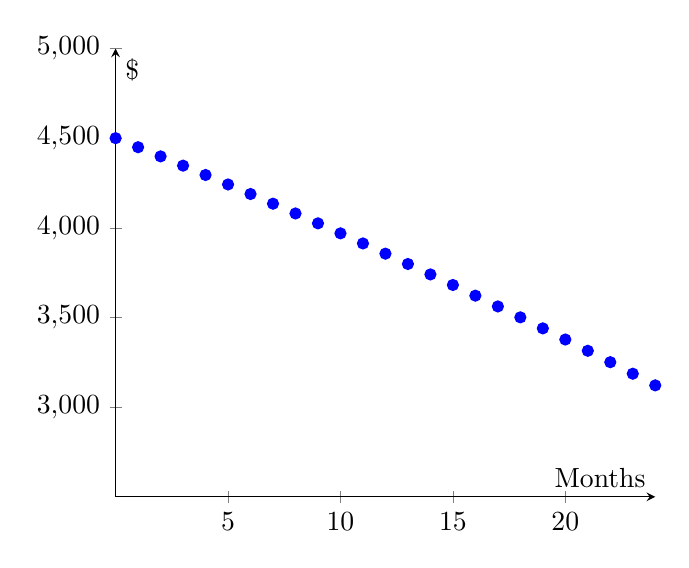
\begin{tikzpicture}
            \begin{axis}[axis lines=center, xmin=0, xlabel={Months}, ymin=2500, ymax=5000,
                ylabel={$\$$}]
                \addplot[mark=*, only marks, blue] coordinates{
                   (0  ,4500.00)
                   (1  ,4449.50)
                   (2  ,4398.44)
                   (3  ,4346.83)
                   (4  ,4294.64)
                   (5  ,4241.88)
                   (6  ,4188.54)
                   (7  ,4134.62)
                   (8  ,4080.10)
                   (9  ,4024.98)
                   (10 ,3969.25)
                   (11 ,3912.92)
                   (12 ,3855.96)
                   (13 ,3798.37)
                   (14 ,3740.16)
                   (15 ,3681.30)
                   (16 ,3621.79)
                   (17 ,3561.63)
                   (18 ,3500.81)
                   (19 ,3439.32)
                   (20 ,3377.15)
                   (21 ,3314.30)
                   (22 ,3250.76)
                   (23 ,3186.52)
                   (24 ,3121.57)};
            \end{axis}
        \end{tikzpicture}
    \end{center}
\end{minipage}

\begin{example}
A student has a college loan of \$$A$ with an interest rate of $r$\% APR compounded monthly.  She pays
$\$p$ per month.  Model the amount that the student owes on the loan with a discrete
dynamical system, examine the behavior of the system based on different values of the
parameter, and give a graph of several numerical solutions.

This situation calls for a discrete dynamical system because the interest and payments are
made in discrete time steps.  Let $a_n$ be a sequence that represents the amount owed on
the loan after $n$ months.  The initial loan amount, \$$A$, is the initial condition, so
\[ a_0 = A. \]
The interest is compounded monthly, so each month the new interest is $r/12\%$ of the
amount owed in the previous month.
\[ \text{new interest} = \frac{r}{12} a_n. \]
The payments are subtracted from the amount owed.  Hence, the mathematical model for the
amount owed on the loan is
\[ \underbrace{a_{n+1}-a_n}_{\text{change in monthly balance}}  = \underbrace{\frac{r}{12}
a_n}_{\text{amount accumulated from interest }} \underbrace{- p}_{\text{payment}}, \quad
\text{where} \quad \underbrace{a_0 = A}_{\text{initial condition}} \]
More simply,
\[ a_{n+1} = a_n + \frac{r}{12} a_n - p \quad \text{where} \quad a_0 = A. \]
Even simpler yet (after a little algebra)
\[ a_{n+1} = \left( 1 + \frac{r}{12} \right) a_n - p. \]
This is a mathematical model for any such situation, and there are many unknown
parameters.  The fact that you don't know the parameters is what makes the problem
interesting!

To discuss the parameters one must think like a scientist; vary one parameter at a time
and try to cover all of the possible bases.  Let us first consider a loan of $A=\$5000$ at
$15\%$ APR.  Figure \ref{fig:9.3.ex1p} shows numerical solutions for several different
payments. Clearly if the payment is larger then the amount of time to pay off the loan
decreases.  
Next let us discuss a different situation.  Assume that the initial loan is still $\$5000$
but now assume that the payments are fixed at $\$200$ and we don't know the rate.  Figure
\ref{fig:9.3.ex1r} shows several numerical solutions to the discrete dynamical system at various rates.

Again, there aren't any real surprises here; as the rate goes down the time to pay off the
loan goes down.  In order to fully explore the parameter space of a discrete dynamical
system (i.e. difference plus initial conditions)  it is easy to
implement the model in Excel and to use absolute cell references for the parameters.  
\end{example}
\begin{figure}[ht!]
    \centering
    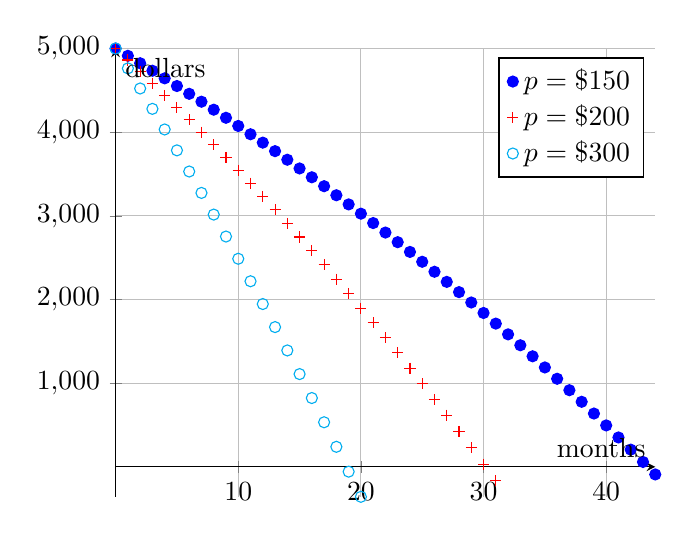
\begin{tikzpicture}
        \begin{axis}[axis lines=center, grid, xlabel={months}, ylabel={dollars}]
            \addplot[blue, mark=*, only marks] coordinates{
(0 , 5000.0)
(1 , 4912.5)
(2 , 4823.9)
(3 , 4734.2)
(4 , 4643.3)
(5 , 4551.4)
(6 , 4458.3)
(7 , 4364.0)
(8 , 4268.5)
(9 , 4171.9)
(10, 4074.1)
(11, 3975.0)
(12, 3874.7)
(13, 3773.1)
(14, 3670.3)
(15, 3566.1)
(16, 3460.7)
(17, 3354.0)
(18, 3245.9)
(19, 3136.5)
(20, 3025.7)
(21, 2913.5)
(22, 2799.9)
(23, 2684.9)
(24, 2568.5)
(25, 2450.6)
(26, 2331.2)
(27, 2210.4)
(28, 2088.0)
(29, 1964.1)
(30, 1838.7)
(31, 1711.6)
(32, 1583.0)
(33, 1452.8)
(34, 1321.0)
(35, 1187.5)
(36, 1052.3)
(37, 915.54)
(38, 776.99)
(39, 636.70)
(40, 494.66)
(41, 350.84)
(42, 205.23)
(43, 57.798)
(44, -91.47)};
\addlegendentry{$p=\$150$};
%
\addplot[red, mark=+, only marks] coordinates{
(0 , 5000.0 )
(1 , 4862.5 )
(2 , 4723.2 )
(3 , 4582.3 )
(4 , 4439.6 )
(5 , 4295.0 )
(6 , 4148.7 )
(7 , 4000.6 )
(8 , 3850.6 )
(9 , 3698.7 )
(10, 3545.0 )
(11, 3389.3 )
(12, 3231.7 )
(13, 3072.0 )
(14, 2910.4 )
(15, 2746.8 )
(16, 2581.2 )
(17, 2413.4 )
(18, 2243.6 )
(19, 2071.6 )
(20, 1897.5 )
(21, 1721.3 )
(22, 1542.8 )
(23, 1362.1 )
(24, 1179.1 )
(25, 993.87 )
(26, 806.30 )
(27, 616.37 )
(28, 424.08 )
(29, 229.38 )
(30, 32.253 )
(31, -167.3 )};
\addlegendentry{$p=\$200$};
%
\addplot[cyan, mark=o, only marks] coordinates{
(0 , 5000.00)
(1 , 4762.50)
(2 , 4522.03)
(3 , 4278.55)
(4 , 4032.03)
(5 , 3782.43)
(6 , 3529.71)
(7 , 3273.84)
(8 , 3014.76)
(9 , 2752.44)
(10, 2486.85)
(11, 2217.93)
(12, 1945.66)
(13, 1669.98)
(14, 1390.85)
(15, 1108.24)
(16, 822.098)
(17, 532.374)
(18, 239.029)
(19, -57.982)
(20, -358.70)};
\addlegendentry{$p=\$300$};
        \end{axis}
    \end{tikzpicture}
    \caption{Numerical solutions to $a_{n+1} = a_n + \frac{r}{12}a_n - p$ with $a_0=5000$
and $r=0.1$ and different values of $p$}
    \label{fig:9.3.ex1p}
\end{figure}

\begin{figure}[ht!]
    \centering
    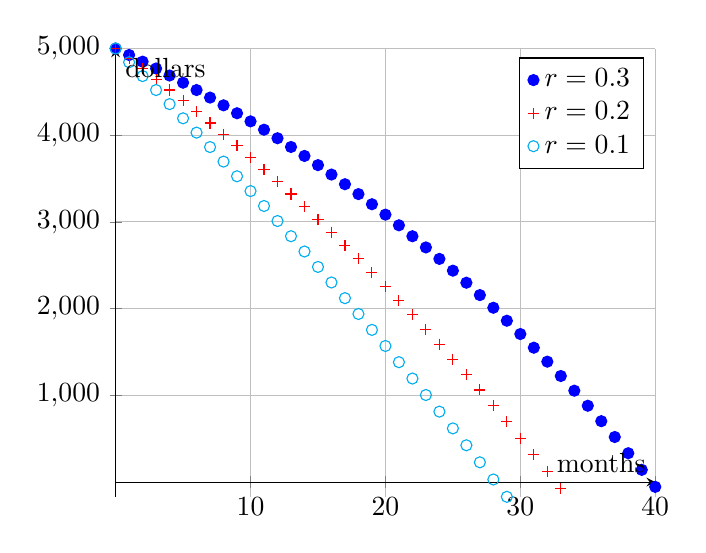
\begin{tikzpicture}
        \begin{axis}[axis lines=center, grid, xlabel={months}, ylabel={dollars}]
            \addplot[blue, mark=*, only marks] coordinates{
(0 , 5000.0)
(1 , 4925.0)
(2 , 4848.1)
(3 , 4769.3)
(4 , 4688.5)
(5 , 4605.7)
(6 , 4520.9)
(7 , 4433.9)
(8 , 4344.7)
(9 , 4253.4)
(10, 4159.7)
(11, 4063.7)
(12, 3965.3)
(13, 3864.4)
(14, 3761.0)
(15, 3655.1)
(16, 3546.4)
(17, 3435.1)
(18, 3321.0)
(19, 3204.0)
(20, 3084.1)
(21, 2961.2)
(22, 2835.2)
(23, 2706.1)
(24, 2573.8)
(25, 2438.1)
(26, 2299.1)
(27, 2156.5)
(28, 2010.5)
(29, 1860.7)
(30, 1707.2)
(31, 1549.9)
(32, 1388.7)
(33, 1223.4)
(34, 1054.0)
(35, 880.38)
(36, 702.39)
(37, 519.95)
(38, 332.95)
(39, 141.27)
(40, -55.19)};
\addlegendentry{$r=0.3$};
\addplot[red, mark=+, only marks] coordinates{
(0 , 5000.0)
(1 , 4883.3)
(2 , 4764.7)
(3 , 4644.1)
(4 , 4521.5)
(5 , 4396.8)
(6 , 4270.1)
(7 , 4141.3)
(8 , 4010.3)
(9 , 3877.2)
(10, 3741.8)
(11, 3604.1)
(12, 3464.2)
(13, 3322.0)
(14, 3177.3)
(15, 3030.3)
(16, 2880.8)
(17, 2728.8)
(18, 2574.3)
(19, 2417.2)
(20, 2257.5)
(21, 2095.1)
(22, 1930.0)
(23, 1762.2)
(24, 1591.5)
(25, 1418.1)
(26, 1241.7)
(27, 1062.4)
(28, 880.16)
(29, 694.83)
(30, 506.41)
(31, 314.85)
(32, 120.10)
(33, -77.89)};
\addlegendentry{$r=0.2$};
\addplot[cyan, mark=o, only marks] coordinates{
(0 , 5000.0)
(1 , 4841.6)
(2 , 4682.0)
(3 , 4521.0)
(4 , 4358.7)
(5 , 4195.0)
(6 , 4029.9)
(7 , 3863.5)
(8 , 3695.7)
(9 , 3526.5)
(10, 3355.9)
(11, 3183.9)
(12, 3010.4)
(13, 2835.5)
(14, 2659.1)
(15, 2481.3)
(16, 2302.0)
(17, 2121.1)
(18, 1938.8)
(19, 1755.0)
(20, 1569.6)
(21, 1382.7)
(22, 1194.2)
(23, 1004.2)
(24, 812.57)
(25, 619.34)
(26, 424.50)
(27, 228.04)
(28, 29.942)
(29, -169.8)};
\addlegendentry{$r=0.1$};
        \end{axis}
    \end{tikzpicture}
    \caption{Numerical solutions to $a_{n+1} = a_n + \frac{r}{12}a_n - p$ with $a_0=5000$
and $p=\$200$ and different values of $r$}
    \label{fig:9.3.ex1r}
\end{figure}
% 



\begin{problem}
    For each of the following situations, create a mathematical model using a difference
    equation or a differential equation.
\ba
\item The population of a town grows at an annual rate of $1.25\%$.
\item A radioactive sample losses $5.6\%$ of its mass every day.
\item  You have a bank account that earns $4\%$ interest every year. At the same time, you
    withdraw money continually from the account at the rate of \$1000 per year.
\item A cup of hot chocolate is sitting in a $70^\circ$ room. The temperature of the hot
    chocolate cools by $10\%$ of the difference between the hot chocolate's temperature and
    the room temperature every minute.
\item A can of cold soda is sitting in a $70^\circ$ room. The temperature of the soda warms at
    the rate of $10\%$ of the difference between the soda's temperature and the room's
    temperature every minute.
    \item Suppose that there are 400 college students living
        in a dormitory and that one or more students has a severe case of the flu.  Assume some
        interaction between those infected and those not infected is required to pass the
        flue.  Assume that a student is either infected or susceptible (no immunities).
        Further assume the number of new infected students each hour is proportional to
        the product of the infected and the susceptible students.  Create a mathematical
        model for the number of infected students over the course of a day.    

        Hint: If there are 400 students in the dorm, then the number of susceptible
        students is 400 minus the number of infected students.
    \item A town has a large reservoir of water that currently contains 450,000 gallons.
        Each week during the spring $W$ gallons are used by the town, while $M$
        gallons flow in from snow melt.  If $r$\% of the water evaporates each week,
        formulate a mathematical model for the amount of water in the reservoir and
        explore the parameter space with the help of Excel. 
        
        Estimates of parameters are as follows: Last year the average water usage during
        the spring was $W=50,000$ gallons and the average intake from snow melt was
        $M=62,500$ gallons.  During the spring the water is estimated to evaporate at
        approximately $1\%$.

%     \item Suppose a national park could support a total population of 3000 bison.  Last
%         year the bison population was 2505, and this year the population grew to 2550.
%         Assume that the bison population is modeled by 
%         \[ b_{n+1} - b_n = k b_n (M-b_n) \]
%         where $M$ is the maximum possible bison population.  Based on the information
%         given, what is the value of $k$
\ea
\end{problem}



\newpage\section{Stability, Equilibria, Phase Plots, and Slope Fields}
\begin{problem}
    Consider the differential equation 
    \[ \frac{dA}{dt} = -0.5A + 0.1. \]
    This model comes from a drug dosing problem where your body removes 50\% of the drug
    every hour and an IV drip administers 0.1mg of drug each hour.  The value of $A$ is
    the number of milligrams of drug in the body at time $t$.  If done correctly, the
    amount of drug in your system will stabilize at a constant level.  What is that level?
    Be sure to fully explain your thinking.
\end{problem}

\begin{problem}
    Consider the difference equation
    \[ A_{n+1} - A_n = -0.2 A_n+ 100. \]
    This model comes from a car sales problem where 20\% of the cars on the lot are sold
    in a given month and 100 new cars are delivered each month.  If you've done things
    correctly as the manager of the lot, the number of cars will stabilize at a certain
    amount.  How many cars is this?  Be sure to fully explain your thinking.
\end{problem}

\begin{problem}
    For each of the two previous problems make a plot with ``change'' on the vertical axis
    and ``amount'' on the horizontal axis.  Each of these should be a linear function just
    like what we saw in the {\it Birth, Death, and Immigration} models.  What is the meaning of
    the ``$x$ intercept'' on each of these plots?
\end{problem}

\begin{problem}
    Return to the {\it Birth, Death and Immigration} models.  You already made a plot with
    ``change'' on the vertical axis and ``population'' on the horizontal axis.  Find the
    point where the linear functions intersect the horizontal axis and interpret these
    points in the context of the problem.
\end{problem}

\begin{definition}[Equilibrium Point]
    An {\bf equilibrium point} in a difference or differential equation is the point where
    the change is 0.
\end{definition}

\begin{example}
    Consider the differential equation $\frac{dy}{dt} = -\frac{1}{2}(y-4)$.  If we set the
    change to zero then we find that 
    \[ 0 = -\frac{1}{2}(y_{eq} - 4) \quad \implies \quad y_{eq} = 4. \]
    The equilibrium is at $y=4$.  Furthermore, if we have a $y$ value a bit less than 4 we
    see that $dy/dt$ is positive so $y$ will be going up.  Also, if we have a $y$ value
    that is a bit more than 4 then $dy/dt$ is negative so $y$ will be going down (see
    Figure \ref{fig:7.2.phase}).  We call this type of equilibrium point {\bf stable}.
\end{example}

\begin{figure}[ht!]
\begin{center}
    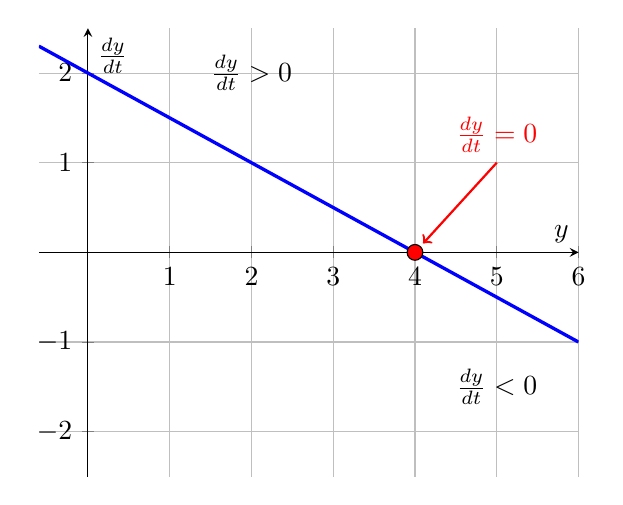
\begin{tikzpicture}
        \begin{axis}[axis lines=center, xmin=-0.6, xmax=6, ymin=-2.5, ymax=2.5, xlabel={$y$},
                ylabel={$\frac{dy}{dt}$}, domain=-0.6:6, grid]
                \addplot[blue, very thick, smooth] {-0.5*(x-4)};
                \draw[fill=red] (axis cs:4,0) circle(0.1cm);
                \draw (axis cs:2,2) node{$\frac{dy}{dt}>0$};
                \draw (axis cs:5,-1.5) node{$\frac{dy}{dt}<0$};
                \draw[thick, red, ->] (axis cs:5,1)
                node[anchor=south]{$\frac{dy}{dt}=0$} -- (axis cs:4.1,0.1);
        \end{axis}
    \end{tikzpicture}\\\vspace{0.1cm}
    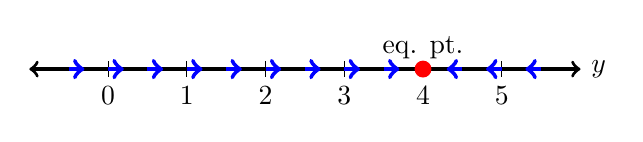
\begin{tikzpicture}
        \draw[very thick, black, <->] (-1,0) -- (6,0) node[anchor=west]{$y$};
        \foreach \j in {0,1,2,3,4,5}{
            \draw (\j,0.1)--(\j,-0.1) node[anchor=north]{$\j$};
        }
        \draw[fill=red, color=red] (4,0) circle(0.1cm);
        \foreach \k in {-0.5,0,0.5,1,1.5,2,2.5,3,3.5}{    
            \draw[ultra thick, blue,->] (\k,0)--(\k+0.2,0);
        }
        \foreach \k in {4.5,5,5.5}{    
            \draw[ultra thick, blue,->] (\k,0)--(\k-0.2,0);
        }
        \draw (4,0) node[anchor=south]{eq. pt.};
    \end{tikzpicture}
\end{center}
\caption{A plot of $\frac{dy}{dt}$ vs $y$ (top) and a phase line diagram (bottom) for the
differential equation $\frac{dy}{dt}=-\frac{1}{2}(y-4)$}
\label{fig:7.2.phase}
\end{figure}

In Figure \ref{fig:7.2.phase} we see two graphical tools that allow us to determine
equilibrium points and their stability.  The top plot in Figure \ref{fig:7.2.phase} is
called a {\bf phase plot} and the bottom plot is called a {\bf phase line}.  In both plots
we can see that $y=4$ is a stable equilibrium.  What this plot doesn't show is what the
{\it solution} to the differential equation actually {\it looks like}.  We only get a
qualitative sense of how the solution behaves from the phase plot and phase line.

Another tool that we have for creating qualitative solutions for differential equations is
the {\bf slope field}.  For every point in the $y-t$ plane we can determine the slope of
the solution to the differential equation by simply putting the $t$ and $y$ into the
right-hand side of the differential equation.  At the point we can then draw a small line
segment with that slope.  If we repeat this process on the differential equation
$\frac{dy}{dt} = -\frac{1}{2} (y-4)$ we get the image in Figure \ref{fig:slope_field_1}.

\begin{figure}[ht!]
    \centering
    \includegraphics[width=0.7\columnwidth]{images/SlopeField_1}
    \caption{A slope field for the differential equation $\frac{dy}{dt} =
    -\frac{1}{2}(y-4)$. }
    \label{fig:slope_field_1}
\end{figure}

\begin{problem}
    In Figure \ref{fig:slope_field_1} you see a slope field for the differential equation
    $\frac{dy}{dt} = -\frac{1}{2} (y-4)$.  
    \begin{enumerate}
        \item[(a)] If you pick an initial condition and draw a
            curve that is tangent to the slope field lines as you draw, then you will end up with
            a rough sketch of a solution to the differential equation.  Draw solutions curves for
            this differential equation using $y(0) = 0, 1, 2, 3, 3.5, 4, 4.5, 5,$ and $6$. 
        \item[(b)] Based on the slope field in Figure \ref{fig:slope_field_1}, your solution plots
            from part (a), and the phase plots in Figure \ref{fig:7.2.phase}, why are we
            classifying the equilibrium at $y=4$ as ``stable''?
    \end{enumerate}
%     Note: It would help to have a printout or a projection of the plot in Figure
%     \ref{fig:slope_field_1} so you can draw directly on it.
\end{problem}

\begin{example}
    Consider the differential equation $\frac{dy}{dt} = \frac{1}{2}(y-4)$.  If we set the
    change to zero then we find that 
    \[ 0 = \frac{1}{2}(y_{eq} - 4) \quad \implies \quad y_{eq} = 4. \]
    The equilibrium is at $y=4$.  Furthermore, if we have a $y$ value a bit less than 4 we
    see that $dy/dt$ is negative so $y$ will be going down.  Also, if we have a $y$ value
    that is a bit more than 4 then $dy/dt$ is positive so $y$ will be going up (see
    Figure \ref{fig:7.3.phase}).  We call this type of equilibrium point {\bf unstable}. A
    slope field for this differential equation can be seen in Figure
    \ref{fig:slope_field_2}.
\end{example}

\begin{figure}[ht!]
\begin{center}
    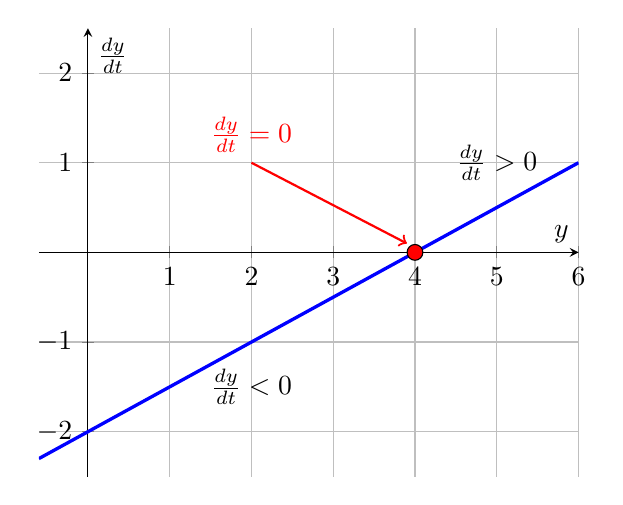
\begin{tikzpicture}
        \begin{axis}[axis lines=center, xmin=-0.6, xmax=6, ymin=-2.5, ymax=2.5, xlabel={$y$},
                ylabel={$\frac{dy}{dt}$}, domain=-0.6:6, grid]
                \addplot[blue, very thick, smooth] {0.5*(x-4)};
                \draw[fill=red] (axis cs:4,0) circle(0.1cm);
                \draw (axis cs:5,1) node{$\frac{dy}{dt}>0$};
                \draw (axis cs:2,-1.5) node{$\frac{dy}{dt}<0$};
                \draw[thick, red, ->] (axis cs:2,1)
                node[anchor=south]{$\frac{dy}{dt}=0$} -- (axis cs:3.9,0.1);
        \end{axis}
    \end{tikzpicture}\\\vspace{0.1cm}
    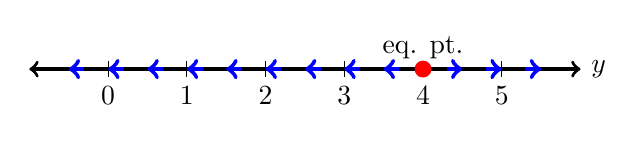
\begin{tikzpicture}
        \draw[very thick, black, <->] (-1,0) -- (6,0) node[anchor=west]{$y$};
        \foreach \j in {0,1,2,3,4,5}{
            \draw (\j,0.1)--(\j,-0.1) node[anchor=north]{$\j$};
        }
        \draw[fill=red, color=red] (4,0) circle(0.1cm);
        \foreach \k in {-0.5,0,0.5,1,1.5,2,2.5,3,3.5}{    
            \draw[ultra thick, blue,<-] (\k,0)--(\k+0.2,0);
        }
        \foreach \k in {4.5,5,5.5}{    
            \draw[ultra thick, blue,<-] (\k,0)--(\k-0.2,0);
        }
        \draw (4,0) node[anchor=south]{eq. pt.};
    \end{tikzpicture}
\end{center}
\caption{A plot of $\frac{dy}{dt}$ vs $y$ (top) and a phase line diagram (bottom) for
$\frac{dy}{dt}=-\frac{1}{2}(y-4)$}
\label{fig:7.3.phase}
\end{figure}

\begin{figure}[ht!]
    \centering
    \includegraphics[width=0.7\columnwidth]{images/SlopeField_2}
    \caption{A slope field for the differential equation $\frac{dy}{dt} =
    \frac{1}{2}(y-4)$. Several solution curves are shown with different initial conditions. }
    \label{fig:slope_field_2}
\end{figure}


\begin{problem}
    We have introduced three big ideas in the past couple of pages.  Let's synthesize some
    of our thinking.  Don't be afraid to look back to the previous examples for
    inspiration.
    \begin{enumerate}
        \item[(a)] To find the equilibrium for a difference or a differential equation,
            set the {\it change} to \underline{\hspace{1in}}.  Explain your answer.
        \item[(b)] When you make a graph of $dy/dt$ vs $y$ (called a phase plot), the
            equilibrium (or equilibria) of the differential equation can be found where
            the curve \underline{\hspace{2in}}. Explain your answer.
        \item[(c)] On a phase line plot you can determine the direction of the arrows by
            looking at the \underline{\hspace{1in}} of the derivative at that value of
            $y$.  Explain your answer.
        \item[(d)] To get the arrows on a slope field, pick a point in the $y-t$ plane and
            \underline{\hspace{2in}}.  
        \item[(e)] To get a solution curve on a slope field, pick an initial condition and
            \underline{\hspace{2in}}.  
    \end{enumerate}
\end{problem}

\begin{problem}
    Find and classify the equilibrium points for each of the following difference or
    differential equations.
\ba
    \item $\displaystyle \frac{dy}{dt} = y(1-y)$
    \item $\displaystyle A_{n+1} - A_n = 2A_n + 6$
    \item $\displaystyle x_{n+1} - x_n = -3x_n - 2$
    \item $\displaystyle \frac{dP}{dt} = -0.5P + 2$
\ea
\end{problem}

\begin{problem}
    Find and classify the equilibrium point for the difference equations modeling the
    three {\it Birth, Death, and Immigration} problems.  Use all of the tools introduced
    in this section.
\end{problem}


\begin{problem}\label{prob:Slope_Fields_Matching}
    In Figure \ref{fig:Slope_Fields_Matching} you will find four slope fields.  Match the
    differential equations below to the slope fields.  Be able to defend your answers.  Once you have matched
    the equations to the slope fields, draw a phase plot and a phase line for each of the
    differential equations.  Finally, classify all of the equilibrium points as stable or
    unstable.
    \begin{flalign*}
        \text{Differential Equation A: } \quad \frac{dy}{dt} &= y(2-y) \\
        \text{Differential Equation B: } \quad \frac{dy}{dt} &= (y-2) \\
        \text{Differential Equation C: } \quad \frac{dy}{dt} &= (2-y) \\
        \text{Differential Equation D: } \quad  \frac{dy}{dt} &= y(2-y)(1-y)
    \end{flalign*}
\end{problem}

\begin{figure}[ht!]
    \centering
    \begin{subfigure}[b]{0.45\textwidth}
        \includegraphics[width=0.95\columnwidth]{images/SlopeField_3}
        \caption{Figure \#1}
    \end{subfigure}
    \begin{subfigure}[b]{0.45\textwidth}
        \includegraphics[width=0.95\columnwidth]{images/SlopeField_6}
        \caption{Figure \#2}
    \end{subfigure}
    \begin{subfigure}[b]{0.45\textwidth}
        \includegraphics[width=0.95\columnwidth]{images/SlopeField_4}
        \caption{Figure \#3}
    \end{subfigure}
    \begin{subfigure}[b]{0.45\textwidth}
        \includegraphics[width=0.95\columnwidth]{images/SlopeField_5}
        \caption{Figure \#4}
    \end{subfigure}
    \caption{Slope fields for Problem \ref{prob:Slope_Fields_Matching}.}
    \label{fig:Slope_Fields_Matching}
\end{figure}

\newpage

\begin{problem}
    What differential equation is associated with the following phase plot? Find the
    equilibrium point and determine its stability.
\begin{center}
    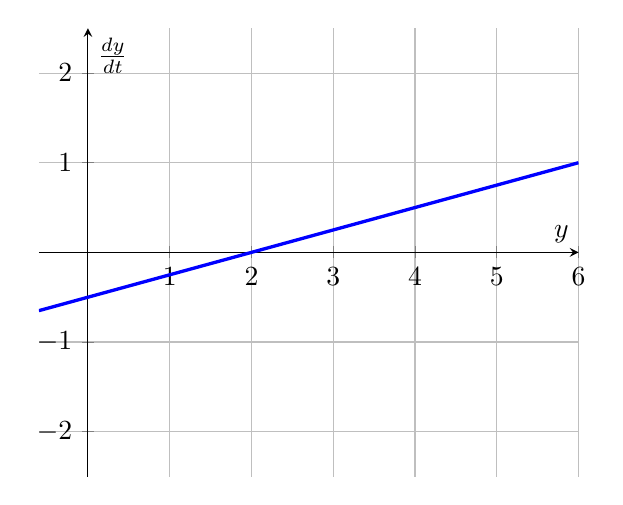
\begin{tikzpicture}
        \begin{axis}[axis lines=center, xmin=-0.6, xmax=6, ymin=-2.5, ymax=2.5, xlabel={$y$},
                ylabel={$\frac{dy}{dt}$}, domain=-0.6:6, grid]
                \addplot[blue, very thick, smooth] {0.25*(x-2)};
%                 \draw[fill=red] (axis cs:4,0) circle(0.1cm);
%                 \draw (axis cs:5,1) node{$\frac{dy}{dt}>0$};
%                 \draw (axis cs:2,-1.5) node{$\frac{dy}{dt}<0$};
%                 \draw[thick, red, ->] (axis cs:2,1)
%                 node[anchor=south]{$\frac{dy}{dt}=0$} -- (axis cs:3.9,0.1);
        \end{axis}
    \end{tikzpicture}
\end{center}
\end{problem}




\begin{technique}[Phase Line Analysis]
    It is often very helpful to draw a {\it phase diagram} (sometimes called a phase line)
    to analyze the equilibrium points of a differential equation.  There are
    four possible cases shown graphically in Figure \ref{fig:phaseline}.  In each of the
    following fill in with the word(s) ``stable'', ``unstable'', ``semi-stable approaching
    from below'', or ``semi-stable approaching from above''.
    \begin{itemize}
        \item In Case \#1 there is a/an \underline{\hspace{1.5in}} equilibrium at $y=2$.
        \item In Case \#2 there is a/an \underline{\hspace{1.5in}} equilibrium at $y=2$.
        \item In Case \#3 there is a/an \underline{\hspace{1.5in}} equilibrium at $y=2$.
        \item In Case \#4 there is a/an \underline{\hspace{1.5in}} equilibrium at $y=2$.
    \end{itemize}
\end{technique}
\solution{
    \begin{itemize}
        \item Case \#1: unstable
        \item Case \#2: semi-stable approaching from below
        \item Case \#3: stable 
        \item Case \#2: semi-stable approaching from above
    \end{itemize}
}

\begin{figure}[h]
    \begin{center}
        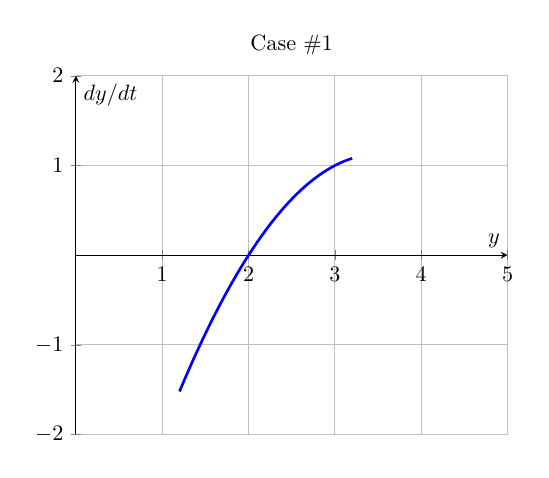
\begin{tikzpicture}[scale=0.8]
            \begin{axis}[axis lines=center, grid, domain=0:5, xlabel={$y$},
                    ylabel={$dy/dt$}, title={Case \#1}, xmin=0, xmax=5, ymin=-2, ymax=2]
                    \addplot[blue, domain=1.2:3.2, very thick, smooth] {-0.5*(x-2)*(x-5)};
            \end{axis}
        \end{tikzpicture}
        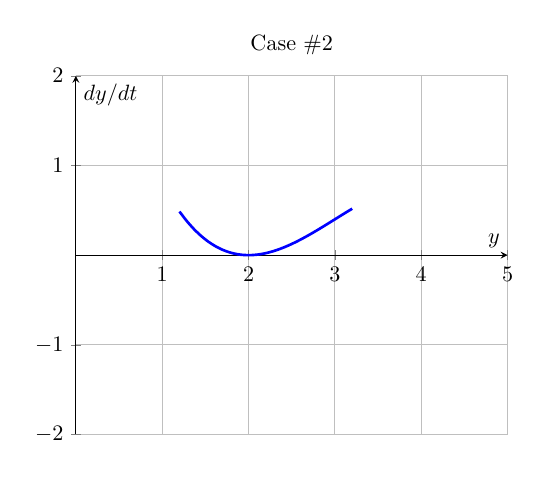
\begin{tikzpicture}[scale=0.8]
            \begin{axis}[axis lines=center, grid, domain=0:5, xlabel={$y$},
                    ylabel={$dy/dt$}, title={Case \#2}, xmin=0, xmax=5, ymin=-2, ymax=2]
                    \addplot[blue, domain=1.2:3.2, very thick, smooth] {-0.2*(x-2)^2*(x-5)};
            \end{axis}
        \end{tikzpicture}
        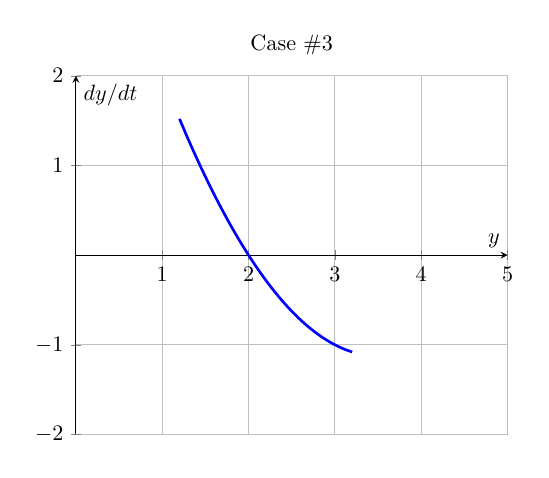
\begin{tikzpicture}[scale=0.8]
            \begin{axis}[axis lines=center, grid, domain=0:5, xlabel={$y$},
                    ylabel={$dy/dt$}, title={Case \#3}, xmin=0, xmax=5, ymin=-2, ymax=2]
                    \addplot[blue, domain=1.2:3.2, very thick, smooth] {0.5*(x-2)*(x-5)};
            \end{axis}
        \end{tikzpicture}
        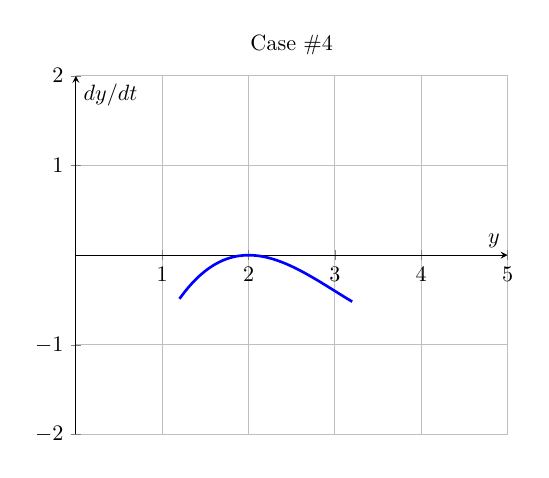
\begin{tikzpicture}[scale=0.8]
            \begin{axis}[axis lines=center, grid, domain=0:5, xlabel={$y$},
                    ylabel={$dy/dt$}, title={Case \#4}, xmin=0, xmax=5, ymin=-2, ymax=2]
                    \addplot[blue, domain=1.2:3.2, very thick, smooth] {0.2*(x-2)^2*(x-5)};
            \end{axis}
        \end{tikzpicture}
    \end{center}
    \caption{Four cases for phase line analysis. In each plot we see a small portion of
        the $\frac{dy}{dt}$ vs $y$ plot for an autonomous first order differential
        equation: $\frac{dy}{dt} = f(y)$.}
    \label{fig:phaseline}
\end{figure}

\newpage


\begin{problem}
    For each of the phase plots in Figure \ref{fig:phase2} sketch a plot on the  $y$ vs
    $t$ plane of the solutions
    to the underlying differential equation with several initial conditions.  At every grid point of the right-hand plots
    draw a small line segment with the slope of the approximate slope of the solution at
    that point.  In the end this will result in the slope field with several solution
    curves..  A few helpful markers are given to
    you in the first plot.
\end{problem}

\begin{figure}[h]
    \begin{center}
        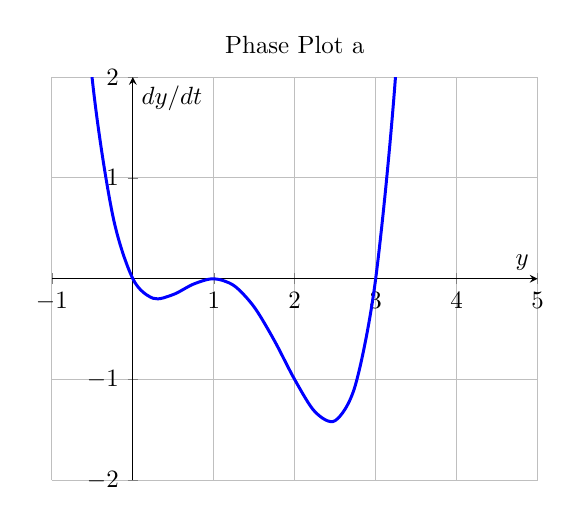
\begin{tikzpicture}[scale=0.9]
            \begin{axis}[axis lines=center, xlabel={$y$}, ylabel={$dy/dt$}, grid, xmin=-1,
                xmax=5, ymin=-2, ymax=2, title={Phase Plot a}]
                \addplot[smooth, very thick, blue, domain=-1:5] {0.5*x*(x-1)^2*(x-3)};
            \end{axis}
        \end{tikzpicture}
        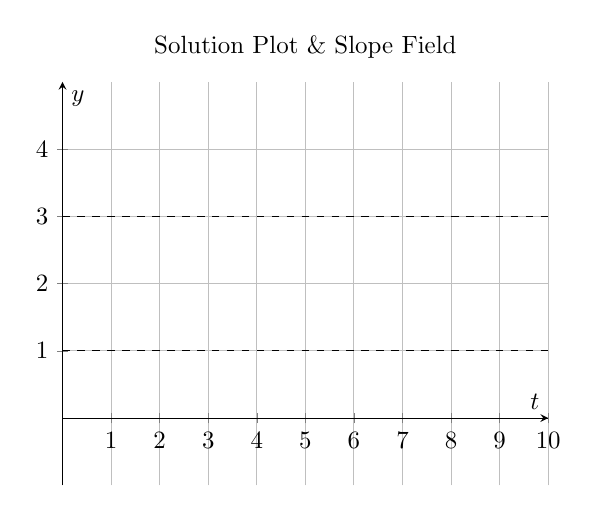
\begin{tikzpicture}[scale=0.9]
            \begin{axis}[axis lines=center, xlabel={$t$}, ylabel={$y$}, grid, xmin=0,
                xmax=10, ymin=-1, ymax=5, title={Solution Plot \& Slope Field}, ytick={1,2,3,4},
            xtick={1,2,3,4,5,6,7,8,9,10}]
                \addplot[dashed, domain=0:10] {0*x+0};
                \addplot[dashed, domain=0:10] {0*x+1};
                \addplot[dashed, domain=0:10] {0*x+3};
            \end{axis}
        \end{tikzpicture}
        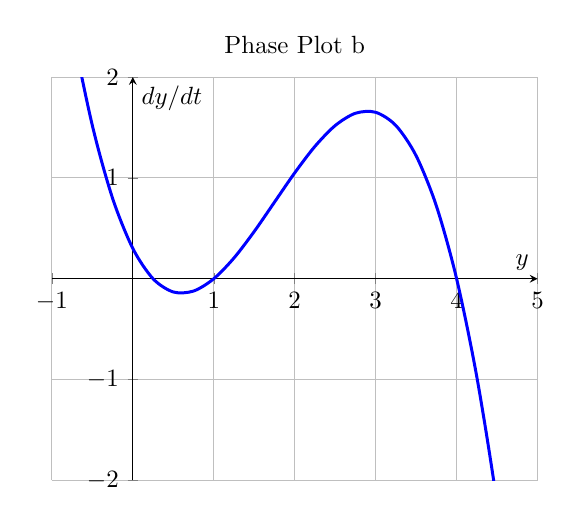
\begin{tikzpicture}[scale=0.9]
            \begin{axis}[axis lines=center, xlabel={$y$}, ylabel={$dy/dt$}, grid, xmin=-1,
                xmax=5, ymin=-2, ymax=2, title={Phase Plot b}]
                \addplot[smooth, very thick, blue, domain=-1:5] {-0.3*(x-0.25)*(x-1)*(x-4)};
            \end{axis}
        \end{tikzpicture}
        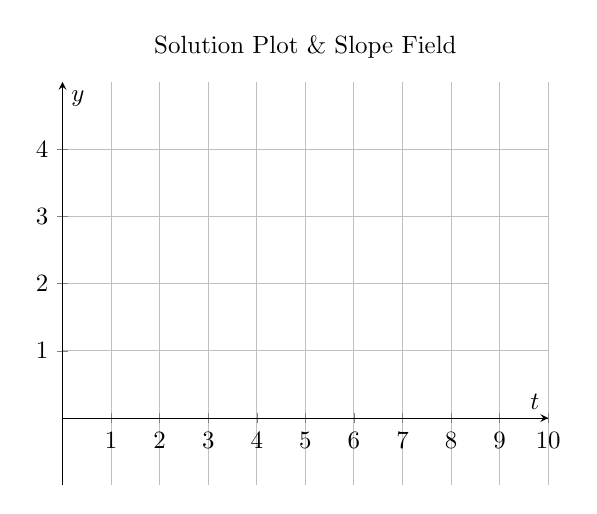
\begin{tikzpicture}[scale=0.9]
            \begin{axis}[axis lines=center, xlabel={$t$}, ylabel={$y$}, grid, xmin=0,
                xmax=10, ymin=-1, ymax=5, title={Solution Plot \& Slope Field}, ytick={1,2,3,4},
            xtick={1,2,3,4,5,6,7,8,9,10}]
                \addplot[smooth, domain=0:10] {0*x+0};
            \end{axis}
        \end{tikzpicture}
    \end{center}
    \caption{Phase plots and solution plots.  On the left are the phase plots and on the
    right are coordinate axes to sketch the solution plots.}
    \label{fig:phase2}
\end{figure}


\begin{problem}
    Use what you learned in the previous problems to find and classify the equilibria for the
    first order non-linear autonomous differential equation
    \[ y'(t) = (y-1)(y-2)(y-3)^2. \]
\end{problem}
\solution{
1 is stable, 2 is unstable and 3 is semi-stable
}


\newpage
\section{Euler's Method: Numerical Solutions for Differential Equations}
One of the fastest ways to get an approximate solution to a difference or a differential
equation is to use technology.  You have already used technology such as MS Excel to build
numerical solutions to difference equations, but what about differential equations?  Let's
look at the two in parallel.  Consider the difference and differential equations
\begin{flalign}
    &\text{difference equation: } a_{n+1} - a_n = -0.5 a_n + 0.1, \text{ and }
    \label{eqn:euler_discrete_ex1} \\
    &\text{differential equation: } \frac{dy}{dt} = -0.5 y + 0.1. 
    \label{eqn:euler_continuous_ex1} 
\end{flalign}
We can turn the differential equation \eqref{eqn:euler_continuous_ex1} into a difference
equation by recalling from Calculus that 
\[ \frac{dy}{dt} \approx \frac{\Delta y}{\Delta t}. \]
Taking $\Delta y = y_{n+1} - y_n$ we arrive at an approximate form of the differential
equation \eqref{eqn:euler_continuous_ex1}
\begin{flalign}
    \frac{y_{n+1} - y_n}{\Delta t} \approx -0.5 y_n + 0.1.
    \label{eqn:euler_continuous_approx}
\end{flalign}
In \eqref{eqn:euler_continuous_approx} we can then rearrange algebraically to get
\begin{flalign}
    y_{n+1} \approx y_n + \Delta t \left( -0.5 y_n + 0.1 \right).
    \label{eqn:euler_continuous_approx2}
\end{flalign}
All we have done at this point is to approximate the derivative $\frac{dy}{dt}$

\begin{problem}
    In MS Excel we are going to solve the difference equation
    \eqref{eqn:euler_discrete_ex1} alongside the differential equation
    \eqref{eqn:euler_continuous_ex1}.  For both we will use the initial condition $a_0 =
    y(0) = 1$.  Notice that these two equations model the same
    behavior with the difference being that the difference equation models in discrete
    time and the differential equations models in continuous time.
    \begin{enumerate}
        \item[(a)] In MS Excel label column \texttt{A} ``Discrete Time'' and label column
            \texttt{B} ``Difference Equation''.  Fill in the times starting at 0 and
            increasing by 1 in column \texttt{A}.  Put the initial condition in cell
            \texttt{B2} and build the difference equation starting in cell \texttt{B3}.
            See the left side of Table \ref{tab:euler_excel}.
        \item[(b)] In the same Excel worksheet label column \texttt{D} ``Continuous Time''
            and label column \texttt{E} ``Differential Equation''.  Put in ``0'' for the
            initial time, choose a time step, and fill in column \texttt{D} with times
            progressing by that time step.  Put the initial condition in cell \texttt{E2}
            and build the approximation to the differential equation
            \eqref{eqn:euler_continuous_approx2} starting at cell \texttt{E3}.
            See the right side of Table \ref{tab:euler_excel}.
        \item[(c)] Fill both numerical solutions so that they end at the same time (the
            continuous time model will obviously be 10 times longer if you use $\Delta t =
            0.1$).  
        \item[(d)] Make a plot showing both solutions on top of each other.
    \end{enumerate}
\end{problem}

\begin{table}[ht!]
    \centering
    \begin{tabular}{|c|c|c|c|c|c|}
        \hline
        & A & B & C & D & E \\
        \hline
        1 & Discrete Time & Difference Equation & & Continuous Time & Differential Equation \\
        \hline 
        2 & 0 & 1 &  & 0 & 1 \\
        3 & 1 & \verb|=B2-0.5*B2+0.1| &  & 0.1 & \verb|=E2+(0.1)*(-0.5*E2+0.2)| \\
        4 & 2 &  &  &  0.2 & \\
        5 & \vdots & \vdots & & \vdots & \vdots \\ \hline
    \end{tabular}
    \caption{Excel setup for a difference equation (left) and differential equation
    (right).}
    \label{tab:euler_excel}
\end{table}


You should have noticed in the previous problem that the solutions to the difference and
differential equations are slightly different than each other.  This is no surprise since
we are taking time steps of ``1'' in the difference equation and we are taking much finer
time steps in the differential equation.  Note further that the only way to make the
approximate solution to the differential equation accurately portray the actual dynamics
of the differential equation we would need to take $\Delta t \to 0$.  Doing so is clearly
infeasible on a computer since we would need infinite memory to do so.  We settle,
instead, for taking $\Delta t$ to be small (0.1 or 0.01 or smaller).  

\begin{definition}[Euler's Method]
    To numerically approximate the solutions to the differential equation
    \[ \frac{dy}{dt} = f(t,y) \]
    we approximate the derivative with 
    \[ \frac{dy}{dt} \approx \frac{y_{n+1} - y_n}{\Delta t} \]
    and use the difference equation
    \[ y_{n+1} = y_n + \Delta t f(t_n,y_n)  \]
    to build an approximate solution.  
\end{definition}
Remember that the only reasonable choice for
$\Delta t$ is to make it {\it very small}.  The trade off to choosing $\Delta t$ small
is that it will take more computer memory to approximate the problem.

A way to think about Euler's method is that at a given point, the slope is approximated by
the value of the right-hand side of the differential equation and then we step forward
$\Delta t$
units in time following that slope.  Figure \ref{fig:Euler} shows a depiction of the idea.
Notice in the figure that in regions of high curvature Euler's method will overshoot the
exact solution to the differential equation.  However, taking $\Delta t \to 0$ theoretically
gives the exact solution at the trade off of needing infinite computational resources.

\begin{figure}[ht!]
    \begin{center}
        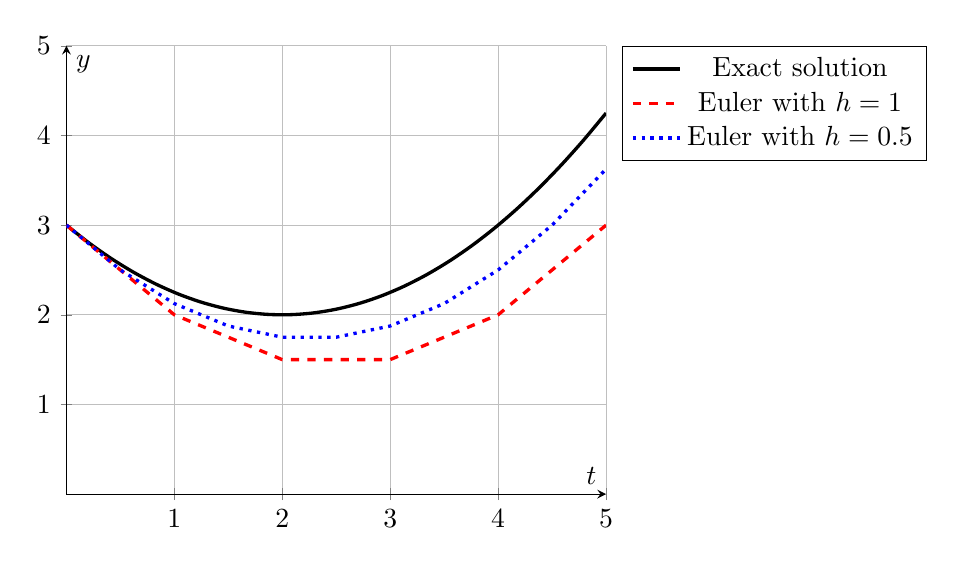
\begin{tikzpicture}
            \begin{axis}[axis lines=center, grid, xmin=0, xmax=5, ymin=0, ymax=5,
                domain=0:5, xlabel={$t$}, ylabel={$y$}, legend pos=outer north east]
                \addplot[very thick, smooth, black] {0.25*(x-2)^2+2};
                \addlegendentry{Exact solution};
                \addplot[red, dashed, very thick]
                coordinates{(0,3)(1,2)(2,1.5)(3,1.5)(4,2)(5,3)};
                \addlegendentry{Euler with $h=1$};
                \addplot[blue, dotted, very thick]
                coordinates{(0,3)(0.5,2.5)(1,2.125)(1.5,1.875)(2,1.75)(2.5,1.75)(3,1.875)(3.5,2.125)(4,2.5)(4.5,3)(5,3.625)};
                \addlegendentry{Euler with $h=0.5$};
            \end{axis}
        \end{tikzpicture}
    \end{center}
    \caption{A depiction of Euler's method with step size $h=1$ (red) and $h=0.5$ (blue).}
    \label{fig:Euler}
\end{figure}


In Figure \ref{fig:Euler_graphical} we see a graphical depiction of how Euler's method
works on the differential equation $y' = y$ with $\Delta t = 1$ and $y(0) = 1$.  The exact
solution to the differential equation is $y(t) = e^t$ and at $t=1$ the solution is $y(1) =
e^1 \approx 2.718$ and is shown in red in the figure. We can see that for large step sizes
Euler's method will drastically miss the true dynamics of the differential equation.

\begin{figure}[ht!]
    \begin{center}
        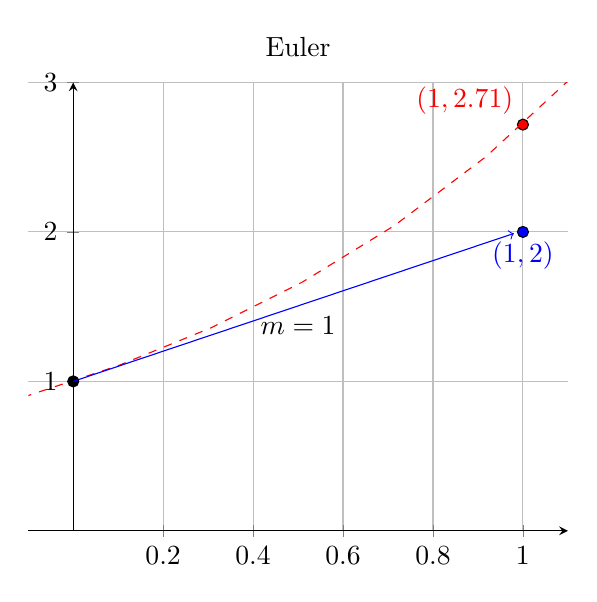
\begin{tikzpicture}
            \begin{axis}[axis lines=center, grid, xmin=-0.1, xmax=1.1, ymin=0, ymax=3,
                title={Euler}]
                \draw[fill=red] (axis cs:1,2.7182) circle(0.07cm); 
                \addplot[dashed, red, samples=50] {1*exp(x)};
                \draw[fill=black] (axis cs:0,1) circle(0.07cm); 
                \draw[blue, ->] (axis cs:0,1) -- (axis cs:0.98,1.99);
                \draw[fill=blue] (axis cs:1,2) circle(0.07cm);
                \draw (axis cs:0.5,1.5) node[anchor=north]{$m=1$};
                \draw[color=blue] (axis cs:1,2) node[anchor=north]{$(1,2)$};
                \draw[color=red] (axis cs:1,2.7182) node[anchor=south east]{$(1,2.71)$};
            \end{axis}
        \end{tikzpicture}
    \end{center}
    \caption{Graphical depiction of Euler's method.  Here we use the simple differential equation
$y'=y$ with $y(0) = 0.5$ and $\Delta t = 1$.  The exact solution is shown in red.}
    \label{fig:Euler_graphical}
\end{figure}



In Excel the process of building an Euler solver is relatively simple.  In \texttt{MATLAB}
it takes a bit more work the very first time, but trust me, the work will pay off in the
long run!  Think carefully about the computer resources necessary to truly capture the
dynamics of a differential equation with Euler's method: very small step size and lots of
computer memory.  In Excel this means lots of dragging with the mouse which is slow,
cumbersome, and annoying.  Let's build the same problem in \texttt{MATLAB}.
\begin{problem}[Euler's Method in MATLAB]
    Open \texttt{MATLAB} and create a new script.  
    The code given below sets up and plots the numerical solution to the problem
    \[ \frac{dy}{dt} = -0.5 y + 0.1. \]
    Explain what each line of code
    does using comments. Some of the lines of code are likely new to you so I suggest you
    either use the help command or you do some basic experimentation.
\begin{lstlisting}
clear; clc; clf;
tmin=0; % define the minimum time
tmax=5; % define the maximum time
dt = 0.1; % what is this line doing?
IC = 1; % define the initial condition for the problem
t=tmin : dt : tmax;  % what does this line do?
y=zeros(size(t)); % what does this line do?
y(1) = IC; % what does this line do?
for n=1:length(t)-1 % what does this line do?
    y(n+1) = y(n) + dt*(-0.5*y(n)+0.1);
end
plot(t,y,'b'), grid on, xlabel('time'), ylabel('y(t)')
title('Euler Approximation')
\end{lstlisting}
\end{problem}

\begin{problem}
    Experiment with different values of $\Delta t$ in your MATLAB code.  I hope that you
    realize that this code is now FAR more flexible than using Excel even though it takes
    a bit more thought to set up at the beginning.
\end{problem}

\begin{problem}
    Modify your Euler's method \texttt{MATLAB} code to get an approximate solution to the differential equation
        \[ y' = -y \cdot \left( 1-\frac{y}{5} \right) + 0.1 t \quad \text{where} \quad
            y(0)=2 \]
\end{problem}

\begin{problem}
    Modify your Euler's method \texttt{MATLAB} code to get an approximate solution to the differential equation
        \[ y' = -y\left( 1-\frac{y}{5} \right)^2 + \sin(t) \]
        for several different initial conditions. Save your plot in an appropriate place
        with appropriate labels and title.
\end{problem}



\begin{problem}
    Solve both of the problems below with MATLAB.  For the difference equation your code
    should be absolutely identical to that of Euler's method with the exception that
    $\Delta t = 1$.  Put the plots on top of each other so you can easily see the
    differences and similarities.
    \begin{flalign*}
        a_{n+1} - a_n &= 0.25 a_n \left( 1 - \frac{a_n}{10} \right) \\
        \frac{dy}{dt} &= 0.25 y \left( 1 - \frac{y}{10} \right). 
    \end{flalign*}
\end{problem}

\begin{problem}
    Go back to every difference and differential equation that we have build thus far in
    this chapter and solve it with both Excel and with MATLAB.
\end{problem}

Save all of the code from both Excel and MATLAB.  We will be using numerical
approximations to solve both difference and differential equations throughout the
remainder of this course.  You will need to be able to build the Euler code in MATLAB
without looking back at old code so take some time in the next few days and practice
writing this code.

% For a complete discussion of Euler's method see the
% \href{http://faculty.gvsu.edu/boelkinm/Home/AC/sec-7-3-euler.html}{Active Calculus book Section
% 7.3}.


\newpage\section{Classifying Difference and Differential Equations}
In order to properly analyze difference equations it is useful to develop a classification
system for all difference and differential equations.  The following definitions describe
several broad classes of difference and differential equations that will be studied in
detail.  These classifications are not merely just names, but they give a hint to the
behavior of the system and the solution techniques.

\begin{definition}[Linear Difference Equations]
    In a {\bf linear} difference equation, the terms that involve sequence variables
    ($a_{n+1}$ or $a_n$) involve no products, no powers, nor functions of sequences
    variables such as exponentials, logarithmic, or trigonometric.  
\end{definition}
\begin{definition}[Linear Differential Equations]
    In a {\bf linear} differential equation, the terms that involve output function $y(t)$
    involve no products, no powers, nor nonlinear functions of $y(t)$ such as exponentials,
    logarithmic, or trigonometric.  
\end{definition}

\begin{definition}[Nonlinear Difference and Differential Equations]
    A difference or differential equation is called {\it non linear} if it is not linear.
\end{definition}
% \begin{problem}
%     Classify each equation as either a difference or differential equation.  Then classify
%     it as either linear or nonlinear
%     \begin{flalign}
%         a_{n+1} - a_n &= 3a_n + n^2 \label{eqn:9.5.ex1a} \\
%         P_{n+1} - P_n &= 5P_n \label{eqn:9.5.ex1b} \\
%         P'(t) &= 5 P(t) \\
%         b'(t) &= (b(t))^2 + 1 \\
%         b_{n+1} - b_n &= (b_n)^2 + 1  \label{eqn:9.5.ex1c} \\
%         a_{n+2} &= a_na_{n+1} \label{eqn:9.5.ex1d} \\
%         f'(t) &= \frac{2}{f(t)}+t \label{eqn:9.5.ex1e} \\
%         a_{n+2} &= a_{n+1} + 3a_n \label{eqn:9.5.ex1f}  \\
%         y'(t) &=  3y(t) + t^2 \label{eqn:9.5.ex1aa} 
%     \end{flalign}
% %     \begin{itemize}
% %         \item Difference equation \eqref{eqn:9.5.ex1a} is linear. 
% %         \item Differential equation \eqref{eqn:9.5.ex1aa} is linear. 
% %         \item Difference equation \eqref{eqn:9.5.ex1b} is linear
% %         \item Difference equation \eqref{eqn:9.5.ex1c} is nonlinear
% %         \item Difference equation \eqref{eqn:9.5.ex1d} is nonlinear
% %         \item Difference equation \eqref{eqn:9.5.ex1e} is nonlinear
% %         \item Difference equation \eqref{eqn:9.5.ex1f} is linear
% %     \end{itemize}
% \end{problem}
% 

\begin{definition}[Homogeneous Difference and Differential Equations]
    A difference or differential equation is called {\bf homogeneous} if the only terms that appear
    in the relationship are ones which involve the output variable (e.g. $a_n$ or
    $a_{n+1}$ in difference equations or $y(t)$ in differential equations).
\end{definition}

\begin{definition}[Nonhomogeneous Equations]
    A difference or differential equation is called {\bf nonhomogeneous} if it is not homogeneous.
\end{definition}

\begin{example}
    Classify each of the following first order models.
    \begin{flalign}
        \frac{dy}{dt} &= y^2 \label{eqn:class1} \\
        b_{n+1} - b_n &= b_n^2 \label{eqn:class2} \\
        x_{n+1} - x_n &= 0.5 x_n + \sin(n) \label{eqn:class3} \\
        \frac{dx}{dt} &= x \sin(t) \label{eqn:class4} 
    \end{flalign}
    {\bf Solution:} \\
    \begin{itemize}
        \item Equation \eqref{eqn:class1} is a first order nonlinear homogeneous
            differential equation.  It is first order because it only contains first
            derivatives.  It is nonlinear because of the square on the $y$ on the
            right-hand side.  It is homogeneous because there is nothing else being added
            to the $y$ term on the right-hand side.
        \item Equation \eqref{eqn:class2} is a first order nonlinear homogeneous
            difference equation.  It is first order because it only contains a difference
            between $b_{n+1}$ and $b_n$.  It is nonlinear because of the square on the
            $b_n$ on the
            right-hand side.  It is homogeneous because there is nothing else being added
            to the $b_n$ term on the right-hand side.
        \item Equation \eqref{eqn:class3} is a first order linear non-homogeneous
            difference equation.  It is first order because it only contains a difference
            between $x_{n+1}$ and $x_n$.  It is linear because the only thing happening to
            the $x_n$ on the right-hand side is multiplication by a scalar.  It is
            non-homogeneous since there is a $\sin(n)$ term added to the right-hand side.
        \item Equation \eqref{eqn:class4} is a first order linear homogeneous
            (non-autonomous) differential equation.  This equation is linear because it
            only contains the first derivative.  It is linear since no non-linear
            functions act on the $x$ on the right-hand side.  This equation is called
            ``non-autonomous'' since there is a ``$t$'' on the right-hand side -- that is,
            the rate depends not only on $x$ but also on $t$.  
    \end{itemize}
\end{example}

\begin{problem}
    Classify the following using the words 
    \begin{itemize}
        \item ``difference equation'' or ``differential equation''
        \item ``linear'' or ``nonlinear''
        \item ``homogeneous'' or ``non-homogeneous''
    \end{itemize}
    If an equation is nonhomogeneous then give the type of function for the
    nonhomogeneity.  For example, the equation $a_{n+1} - a_n = 0.5 a_n + 10$ is a linear
    nonhomogeneous difference equation with a constant nonhomogeneity.
    \begin{flalign}
        a_{n+1} - a_n &= 3a_n + n^2 \\
        P_{n+1} - P_n &= 5P_n \\
        P'(t) &= 5 P(t) \\
        b'(t) &= (b(t))^2 + 1 \\
        b_{n+1} - b_n &= (b_n)^2 + 1  \\
        a_{n+2} &= a_na_{n+1} \\
        f'(t) &= \frac{2}{f(t)}+t \\
        a_{n+2} &= a_{n+1} + 3a_n \\
        y'(t) &=  3y(t) + t^2 
    \end{flalign}
\end{problem}


\newpage\section{Technique: Solving $1^{st}$ Order Linear Homogeneous Equations}
In this section we will solve the most basic difference and differential equations.  
\begin{flalign}
    a_{n+1} - a_n &= r a_n \quad \text{with initial condition} \quad a_0 
    \label{eqn:1st_order_hom_difference} \\
    y'(t) &= r y(t) \quad \text{with initial condition} \quad y(0) = y_0.
    \label{eqn:1st_order_hom_differential}
\end{flalign}
The reader should note that \eqref{eqn:1st_order_hom_difference} is a linear homogeneous
difference equation and \eqref{eqn:1st_order_hom_differential} is a linear homogeneous
differential equation. These solution techniques will be the basis for all future solution
techniques so take careful note of the techniques \ldots we'll use them a lot!!

\begin{problem}
We wish to solve the difference equation $a_{n+1} - a_n = ra_n$ with initial condition $a_0$.  
Fill in the blanks in the following table to arrive at an analytic solution to this
difference equation.
\begin{center}
    \begin{tabular}{|c|l|}
        \hline
        $n$ & $a_n$ \\ \hline \hline
        $0$ & $a_0$ \\
        $1$ & $a_1 = \underline{\hspace{0.4in}} a_0$ \\
        $2$ & $a_2 = \underline{\hspace{0.4in}} a_1 =  \underline{\hspace{0.4in}}a_0$ \\
        $3$ & $a_3 = \underline{\hspace{0.4in}}a_2  = \underline{\hspace{0.4in}}a_0$ \\
        $4$ & $a_4 = \underline{\hspace{0.4in}}a_3 =  \underline{\hspace{0.4in}}a_0$ \\
        $\vdots$ & $\vdots$ \\
        $k$ & $a_k =  \underline{\hspace{0.4in}}a_0$ \\ \hline
    \end{tabular}
\end{center}
\end{problem}

Your work in the previous problem has just provided sufficient evidence to believe following theorem. 
\begin{thm}\label{thm:9.6.linearhom}
    If $a_{n+1} - a_n = ra_n$ with initial condition $a_0$ then the analytic solution to
    the discrete dynamical system is
\begin{flalign}
    a_k = \underline{\hspace{0.4in}} \cdot a_0.
    \label{eqn:9.6.lienarhom_soln}
\end{flalign}
\end{thm}

\begin{problem}
    Returning now to the original difference equation from this chapter, find the solution
    to the difference equation
    \[ P_{n+1} - P_n = -0.5 P_n \]
    with initial condition $P_0 = 50$.  Use Excel to make a plot of the analytic solution
    along with a numerical solution.
\end{problem}


Now let's solve equation \eqref{eqn:1st_order_hom_differential}.  To do this we'll need to
make a simple observation about calculus.
\begin{problem}
    There are two functions that have the property that they are equal to their
    derivative. Both of these equations solve the differential equation $y'(t) = y(t)$.
    The first solution is the function $y(t) = 0$ since $\frac{d}{dt}(0) = 0$.  What
    is the other solution function?
\end{problem}

Now let's solve almost the exact same differential equation: $y'(t) = ry(t)$.  
\begin{problem}
    Based on your answer to the previous problem, what is the solution to the differential
    equation $y'(t) = ry(t)$?
\end{problem}
You should notice that in both the difference equation, $a_{n+1} - a_n = ra_n$, and the
differential equation, $y(t) = ry(t)$, the solution turns out to be exponential.
The only big difference is the base of the exponential.  

\begin{thm}
    The solution to the differential equation $y'(t) = ry(t)$ with initial condition $y(0)
    = y_0$ is
    \[ y(t) = \underline{\hspace{1in}}. \]
\end{thm}


\begin{problem}
    Solve the following first order homogeneous difference and differential equations.
    \begin{flalign*}
        a_{n+1} - a_n &= 3 a_n \quad \text{with} \quad a_0 = 7 \\ 
        y'(t) &= 3 y(t) \quad \text{with} \quad y(0) = 7 \\ 
        b_{n+1} - b_n &= -0.3 b_n \quad \text{with} \quad b_0 = 7 \\ 
        x'(t) &= -0.3 x(t) \quad \text{with} \quad x(0) = 2 
    \end{flalign*}
\end{problem}

\begin{problem}
    Write a mathematical model associated with each of the previous equations.
\end{problem}

\newpage\section{Technique: Solving $1^{st}$ Order Linear Nonhomogeneous Equations}
We now turn to finding analytic solutions to the difference equations and differential
equation that we've encountered thus far.   We will start with a technique, called {\it
separation of variables}, that only applies to differential equations since in
differential equation we can leverage the ideas of calculus.   We will then look at a
powerful technique called {\it the method of undetermined coefficients} that works for
both differential equations and difference equations.  With practice you'll get the hang
of which one to use in which instances.

\subsection{Solution Technique: Separation of Variables}
\begin{problem}
    Consider the differential equation 
    \[ \frac{dy}{dt} = y \]
    with the initial condition $y(0) = 1$.
    \begin{enumerate}
        \item[(a)] Putting the differential equation into words: \\ {\it the derivative of
            some unknown function is equal to the function itself.} \\
            what is the function?
        \item[(b)] Allow me to abuse some notation: \\
            If you multiply both sides by $dt$ and divide both sides by $y$ we end up with
            \[ \frac{dy}{y} = dt. \]
            Integrate both sides and solve for $y$. Don't forget the arbitrary constants
            resulting from indefinite integrals.
        \item[(c)] Compare your answers to parts (b) and (c).
    \end{enumerate}
\end{problem}
\solution{
The solution is clearly $y(t) = e^t$.
}

\begin{problem}
    In part (b) of the previous problem we said that we were ``abusing notation''.  What does
    that mean?  What notation is being abused?
\end{problem}

\begin{technique}[Separation of Variables]
    To solve a differential equation of the form
    \[ \frac{dy}{dx} = f(y)\cdot g(x) \]
    Separate and integrate by treating the ``$dy/dt$'' as a fraction\footnote{Technically
        speaking the ``$dy/dt$'' is not a fraction it is a shorthand notation for a
    limit.  More technically there is some sneaky chain rule happening behind the scenes
here \ldots can you find it.}
    \[ \int \frac{dy}{f(y)} = \int g(x) dx \]
    Notice that the right-hand side of the differential equation factors perfectly hence
    separating the variables into the functions $f$ and $g$.
\end{technique}

\begin{problem}
    With your partner, write a differential equation that can be solved via separation of
    variables.  Once you have your equation trade with a different group and solve their
    equation.
\end{problem}

\begin{example}
    Solve the differential equation 
    \[ \frac{dy}{dt} = 0.5 y \quad \text{with} \quad y(0) = 7 \]
    using the method of separation of variables.\\{\bf Solution:} Notice that this
    differential equation is separable since we can separate the functions of $y$ and the
    functions of $t$
    \[ \frac{dy}{y} = 0.5 dt. \]
    Integrating both sides of this equation we get
    \[ \int \frac{1}{y} dy = \int 0.5 dt \quad \implies \quad \ln(y) + C_1 = 0.5 t + C_2.
    \]
    Notice that if we subtraction the constant $C_1$ from both sides we actually just get
    a new arbitrary constant on the right-hand side.  For this reason it is customary to
    only write one of the two constants when showing the work for this method
    \[ \ln(y) = 0.5 t + C. \]
    Exponentiating both sides of this equation gives 
    \[ y(t) = e^{0.5 t + C} \]
    and we can now recognize that this is the same, algebraically, as
    \[ y(t) = e^{0.5t} e^C.  \]
    Furthermore, $e^C$ is just another constant so we write the general solution as 
    \[ y(t) = Ce^{0.5t}. \]
    To get the value of $C$ we substitute $t=0$ into the equation to get $7 = Ce^0$ which
    implies that $C= 7$ and the solution is 
    \[ y(t) = 7e^{0.5t}. \]
\end{example}

\begin{example}
    Solve the differential equation 
    \[ \frac{dy}{dt} = 3y+12 \quad \text{with} \quad y(0) = 2 \]
    using separation of variables. \\{\bf Solution:} We're first going to factor the
    right-hand side of the differential equation so that the integration that we run in to
    is not so hard.
    \[ \frac{dy}{dt} = 3(y+4). \]
    Separating and integrating gives
    \[ \int \frac{1}{y+4} dy = \int 3dt \quad \implies \quad \ln(y+4) = 3t+C. \]
    Exponentiating both sides and repeating the same type of algebra as in the previous
    example we get
    \[ y + 4 = Ce^{3t}. \]
    Finally, we can subtract 4 from both sides of the equation to get the general solution
    \[ y(t) = Ce^{3t} - 4. \]
    Using the initial condition we see that 
    \[ 2 = C - 4 \quad \implies \quad C=6 \]
    which implies that 
    \[ y(t) = 6 e^{3t} - 4. \]
\end{example}


\begin{problem}
    A drug is eliminated from the body via natural metabolism.  Assume that there is an
    initial amount of $A_0$ drug in the body.  Which of the following is the best
    differential equation model for the drug removal?  Once you have the model solve it
    with the appropriate technique.
    \begin{enumerate}
        \item $A' = -kt$
        \item $A' = -kA$
        \item $A' = -kA\left( 1-\frac{A}{A_{max}} \right)$
        \item $A' = -kAt$
    \end{enumerate}
\end{problem}
\solution{
    $A'=-kA$ so $A(t) = Ce^{-kt}$ with separation of variables.  \\ Show a slope field for
    this and discuss stability and equilibrium. Also discuss why the other won't work.
}

\begin{problem}
    An ideal ice cube that is exactly cube shaped (perfect squares on all sides) melts in
    your drink.  A differential equation that models the melting of the ice is 
    \[ \frac{dV}{dt} = k S(t) \]
    where $S(t)$ is a function describing the surface area of the ice cube.  
    \begin{enumerate}
        \item[(a)] Explain why this differential equation is physically reasonable.
        \item[(b)] Write down the geometric formulas for the volume and the surface area
            of a cube in terms of the length of the side, $x$:
            \[ V(x) = \underline{\hspace{1in}} \qquad S(x) = \underline{\hspace{1in}} \]
        \item[(c)] Solve the surface area function for $x$ as a function of $S$.
        \item[(d)] Substitute your answer from part (c) into the $x$ in the volume
            equation in part (b). 
        \item[(e)] Rewrite the differential equation 
            \[ \frac{dV}{dt} = kS \]
            in terms of $V$ using your answer from part (d).
        \item[(f)] Solve the differential equation resulting from part (e) using
            separation of variables.
    \end{enumerate}
\end{problem}


\begin{problem}
    Suppose that a cup of coffee is initially at a temperature of $105^\circ$ F and is
    placed in a $75^\circ$ F room.  Newton's law of cooling says that 
    \[ \frac{dT}{dt} = -k\left( T - 75 \right) \]
    where $k$ is a constant related to the insulation properties of the coffee mug.  
    \begin{enumerate}
        \item[(a)] Suppose you measure that the coffee is cooling at one degree per minute
            at the time the coffee is brought into the room.  Use the differential
            equation to determine the value of the constant $k$.
        \item[(b)] Find all solutions to this differential equation.
        \item[(c)] What happens to all of the solutions as $t\to\infty$?  Explain how this
            agrees with your intuition.
        \item[(d)] What is the temperature of the cup of coffee after 20 minutes?
        \item[(e)] How long does it take for the coffee to cool to $80^\circ$F?
    \end{enumerate}
\end{problem}

\begin{problem}
    In a dog, an intravenous dose of 30 mg of pentobarbital sodium per kilogram of body
    weight will usually produce surgical anesthesia. Also in the dog, pentobarbital has a
    biological halflife of about 4.5 hours, due almost entirely to metabolism.  You
    anesthetize a 14-kg dog with the above dose of pentobarbital. Two hours later the
    anesthesia is obviously beginning to lighten and you want to restore the original
    depth of anesthesia. How many milligrams of pentobarbital sodium should you inject?
    Write and solve a differential equation to answer this question.
\end{problem}
\solution{
    The simplest differential equation model is 
    \[ \frac{dP}{dt} = -kP \]
    where $P$ is the amount of pentobarbital (in mg) and $t$ is time (in hours).  The
    solution is clearly $P(t) = C e^{-kt}$ where $C = 420 = (14 \text{kg})(30
    \text{mg/kg})$.  Since we know the half life of the drug we can find $k$ as
    \[ 0.5P_0 = P_0 e^{-k(4.5)} \quad \implies \quad k \approx 0.154033 \]
    and hence $P(t) = 420 e^{-0.15033t}$.
}


\begin{problem}
    In a local pine forest the Pine Beetle is killing the trees at a rate proportional to the
    number of available trees in the forest.  A conservation group is attempting to curb the
    problem by planting 5 live trees per week.  Write a differential equation describing
    this scenario, classify the differential equation, and determine if it can be solved
    with separation of variables.
%     Which of the following is a mathematical model
%     for the number of live trees as a function of time (measured in weeks)?
%     \begin{enumerate}
%         \item $T' = -kT + 5$
%         \item $T' = -kT + 5*t$
%         \item $T' = -5k*T*t$
%         \item $T' = -5k*t$
%     \end{enumerate}
\end{problem}
\solution{
$T' = -kT + 5$.  First order, linear, autonomous, non-homogeneous. Separation is fine
since is it autonomous.
\[ \int \frac{dT}{T-5/k} = \int -k dt = -kt+C \implies \ln(T-5/k) = -kt+C \implies T =
Ce^{-kt} + \frac{5}{k} \]
}


\begin{problem}
    Solve each of the following differential equations.  If an initial condition is given
    then use it to find any unknown constants. (Some of these may require advanced
    integration techniques)
    \begin{flalign*}
        \frac{dy}{dt} - (2-t)y &= 2-t \\
        \frac{1}{t} \frac{dy}{dt} &= e^{t^2-2y} \\
        \frac{dy}{dt} &= 2y+2,\, y(0) = 2 \\
        \frac{dy}{dt} &= 2y^2, \, y(-1) = 2
    \end{flalign*}
\end{problem}

We'll wrap up this subsection with a few more examples.
\begin{example}
    Solve the differential equation
    \[ \frac{dy}{dt} = \frac{y}{t^2} \quad \text{with} \quad y(1) = 5 \]
    using separation of variables.  \\{\bf Solution:} We can separate variables,
    integrate, and do some algebra to get
    \[ \int \frac{dy}{y} = \int \frac{dt}{t^2} \quad \implies \quad \ln(y) =
    -\frac{1}{t} + C \quad \implies \quad y(t) = Ce^{-1/t}. \]
    Using the condition $y(1) = 5$ we see that $5 = Ce^{-1}$ which implies that $C = 5e$
    and the solution to the differential equation is 
    \[ y(t) = 5e^{1-1/t}. \]
\end{example}

\begin{example}
   Solve the differential equation 
   \[ \frac{dy}{dt} = \frac{2ty}{t^2+1} \]
   using separation of variables. \\{\bf Solution:}
   If we separate the variables and integrate we see that 
   \[ \int \frac{dy}{y} = \int \frac{2t}{t^2+1} dt \quad \implies \quad \ln(y) =
   \ln(t^2+1)+C. \]
   The right-hand integral used the idea of $u$-substitution (you should stop now and work
   out the $u$-substitution by hand).  Exponentiating both sides gives
   \[ y(t) = e^{\ln(t^2+1)+C} = Ce^{\ln(t^2+1)} = C(t^2+1). \]
\end{example}

For more problems related to separation of variables see
\href{https://activecalculus.org/single/sec-7-4-separable.html}{Active Calculus Section
7.3}.  


% \begin{problem}
%     True or False: Every first order autonomous differential equation is separable. Be
%     able to defend your answer.
% \end{problem}
% \solution{True, but the integration may be horrible!}
% 
% 
% \begin{problem}
%     In the movie Interstellar, ``Plan B'' was for the astronauts to start a colony on a new
%     planet.  There was 1 female in the group so she would presumably carry the children.
%     Genetic diversity was no problem because of the donor eggs.  The supplies on the colony
%     would be limited by local resources as well as what they brought with them
%     (which minimal).  Which of the following models should the astronauts use to plan
%     their future reproduction, and what do the parameters mean?  Explain your choice for the best one.
%     \begin{itemize}
%         \item $P' = kP$
%         \item $P' = kt$
%         \item $P' = -kP\ln(P/N)$
%         \item $P' = kP(1-P/N) $
%     \end{itemize}
% \end{problem}
% \solution{A logistic model is the best choice. Either of the last two choice could work.
%     \[ \int \frac{dP}{P\ln(P/N)} = \int -k dt \implies \int \frac{dP}{P\ln(P/N)} = -kt + C
%     \]
%     \[ \implies (\text{with } u=P/N) \,  \int \frac{1}{u\ln(u)} = -kt+C \implies
%     (\text{with } v=1/u) \, \int \frac{1}{v}dv = -kt + C \]
%     \[ \implies \ln(v) = -kt+c \implies \ln(\ln(P/N))=-kt+C \implies \ln(P/N) = Ce^{-kt}
%     \implies P(t) = N e^{Ce^{-kt}} \]
% 
%     For the more standard logistic model:
%     \[ \int \frac{dP}{P(1-P/N)} = -kt+C \implies \int \frac{A}{P} + \frac{B}{1-P/N} dP =
%     -kt + C \implies \int \frac{1}{P} + \frac{(1/N)}{1-P/N} dP = -kt+ C \]
%     \[ \implies \ln(P) - \ln(1-P/N) = -kt+C \implies \ln \left( \frac{P}{1-P/N} \right) =
%     -kt+C\]
%     \[ \implies \frac{P}{1-P/N} = Ce^{-kt} \implies P(t) = \frac{Ce^{-kt}}{1-Ce^{-kt}/N}
%     \]
% 
% }
% 

\subsection{Solution Technique: Undetermined Coefficients}
Now let's focus on a solution technique that works for both difference and differential
equations.  When faced with a separable differential equation you'll find that separation
of variables will always be easier.  However, not all differential equations are
separable!  For example, the differential equation $y' = 0.5y + t$ cannot be separated.
Furthermore, separation of variables makes no sense on difference equations since there
are no derivatives.

% Some folks call this technique the ``four step method'', but in reality this is just one
% of many techniques for solving non-homogeneous differential equations.  Instead of
% thinking of this in ``four steps'' you should really just consider this a bit of
% mathematical detective work.  
You can think of this new method, {\it the method of undetermined coefficients}, as {\it
mathematical detective work}.  We're going to guess the form of the solution and then
follow our noses to find the missing coefficients -- hence the name {\it undetermined
coefficients}.  

\begin{technique}[Undetermined Coefficients]
    The method of {\it undetermined coefficients} is roughly outlined as:
    \begin{enumerate}
        \item find a solution for the homogeneous equation,
        \item conjecture a particular solution for the non-homogeneous equation, 
        \item use the initial condition to find a relationship between some of the
            coefficients, and
        \item use the particular solution in the equation to find the
            remaining coefficients.
    \end{enumerate}
\end{technique}

We'll highlight this technique with a sample problem.  Work through all of these steps to
get the idea of how to use undetermined coefficients.
\begin{problem}
    Solve the following first order linear non-homogeneous differential equation by
    following the steps outlined.
    \[ \frac{dy}{dt} = -0.2 y + 3 \quad \text{with} \quad y(0) = 5 \]
    \begin{enumerate}
        \item[(a)] First solve the homogeneous part of the equation: $y' = -0.2y$.  Don't
            use the initial condition yet.
            \[ y_{hom}(t) = \underline{\hspace{1in}} \]
            \solution{$y_h(t) = C_0 e^{-0.2t}$}
        \item[(b)] Next conjecture that a {\it particular} solution has the same functional
            form as the non-homogeneity.  In this case the non-homogeneity is a constant
            function so we guess that the particular function is a generic constant
            function
            \[ y_{particular}(t) = C. \]
        \item[(c)] The full analytic solution to the differential equation is the sum of the
            homogeneous and particular solutions: $y(t) = y_{hom}(t) + y_{part}(t)$.  Note
            that this is only the case for linear difference or differential equations.
            \[ y(t) = \underline{\hspace{2in}} \]
            \solution{$y(t) = C_0 e^{-0.2t} + C_1$}
        \item[(d)] Substitute the particular solution into the differential equation and see
            what equation comes out
            \[ \underline{\hspace{1in}} = \underline{\hspace{1in}} \]
            \solution{$0=-0.2C_1+3 \implies C_1 = 3/0.2=15$ }
        \item[(e)] Substitute the initial condition into the analytic solution and see what
            equation comes out
            \[ \underline{\hspace{1in}} = \underline{\hspace{1in}} \]
            \solution{$5=C_0 + 15 \implies C_0 = -10$ }
        \item[(f)] Determine the final solution
            \solution{$y(t) = -10e^{-0.2t} + 15$}
    \end{enumerate}
\end{problem}

\begin{problem}
    Leave all of your work from the previous problem somewhere you can see it.  We're now
    going to solve a difference equation of the exact same form using the method of
    undetermined coefficients. \\
    Solve the difference equation
    \[ a_{n+1} - a_n = -0.2 a_n + 3 \quad \text{with} \quad a_0 = 5. \]
    \begin{enumerate}
        \item[(a)] First solve the homogeneous part of the equation: $a_{n+1} - a_n = -0.2
            a_n$. Don't use the initial condition yet. 
            \[ a_{hom} = \underline{\hspace{1in}} \]
            \solution{
                \[ a_{hom} = C (1-0.2)^n. \]
            }
        \item[(b)] Next conjecture that a {\it particular} solution has the same functional
            form as the non-homogeneity.  In this case the non-homogeneity is a constant
            function so we guess that the particular function is a generic constant
            function
            \[ a_{particular} = C. \]
        \item[(c)] The full analytic solution to the differential equation is the sum of the
            homogeneous and particular solutions: $a_n = a_{hom} + a_{part}$.  Note
            that this is only the case for linear difference or differential equations.
            \[ a_n = \underline{\hspace{2in}} \]
            \solution{$a_n = C_0 (0.8)^n + C_1$}
        \item[(d)] Substitute the particular solution into the difference equation and see
            what equation comes out
            \[ \underline{\hspace{1in}} = \underline{\hspace{1in}} \]
            \solution{$0=-0.2C_1+3 \implies C_1 = 3/0.2=15$ }
        \item[(e)] Substitute the initial condition into the analytic solution and see what
            equation comes out
            \[ \underline{\hspace{1in}} = \underline{\hspace{1in}} \]
            \solution{$5=C_0 + 15 \implies C_0 = -10$ }
        \item[(f)] Determine the final solution
            \solution{$a_n = -10 (0.8)^n + 15$}
    \end{enumerate}
\end{problem}

\begin{problem}
    Time for a compare and contrast.  Put the solutions to both of the previous two
    problems somewhere you can see both of them.  Compare and contrast the steps.  Once
    you've convinced yourself that there is essentially no difference in the technique for
    either difference or differential equations, plot both equations on the same
    coordinate plane and discuss the similarities and differences. Where did the
    differences come from? 
\end{problem}


\begin{technique}[Undetermined Coefficients]
    To solve a non-homogenous linear difference or differential equation:
    \begin{enumerate}
        \item Solve the associated homogeneous equation.
        \item Conjecture a {\it particular solution} that has the same functional form as
            the non-homogeneity.
        \item Build the full analytic solution as a linear combination of the homogeneous and
            particular solutions.
        \item Substitute the particular solution into the difference or differential equation.
        \item Substitute the initial condition(s) into the analytic solution.
        \item Use the equations that you found in steps 4 and 5 to find the constants.
    \end{enumerate}
\end{technique}

\begin{problem}\label{prob:undet_coeff}
    For each of the following linear non-homogeneous difference or differential equations
    write the homogeneous solution and the particular solution. 
    \begin{enumerate}
        \item[(a)] $y' = 3y + 4$ \qquad $y_{hom}(t) = \underline{\hspace{1in}}$\, and\, $y_{part}(t) = \underline{\hspace{1in}}$
        \item[(b)] $a_{n+1} - a_n = 3a_n + 4$ \qquad $a_{hom} =
            \underline{\hspace{1in}}$\, and\, $a_{part} = \underline{\hspace{1in}}$
        \item[(c)] $y' = 3y + 4t$\qquad $y_{hom}(t) = \underline{\hspace{1in}}$\, and\, $y_{part}(t) = \underline{\hspace{1in}}$
        \item[(d)] $a_{n+1}-a_n = 3a_n + 4t$\qquad $a_{hom} =
            \underline{\hspace{1in}}$\, and\, $a_{part} = \underline{\hspace{1in}}$
        \item[(e)] $y' = 3y + 4\sin(t)$\qquad $y_{hom}(t) = \underline{\hspace{1in}}$\,
            and\, $y_{part}(t) = \underline{\hspace{1in}}$
        \item[(f)] $a_{n+1} - a_n = 3a_n + 4\sin(n)$\qquad $a_{hom} = \underline{\hspace{1in}}$\,
            and\, $a_{part} = \underline{\hspace{1in}}$
        \item[(g)] $y' = 3y + 4e^{-t}$\qquad $y_{hom}(t) = \underline{\hspace{1in}}$\,
            and\, $y_{part}(t) = \underline{\hspace{1in}}$
        \item[(h)] $a_{n+1} - a_n = 3a_n + 4e^{-n}$\qquad $a_{hom} = \underline{\hspace{1in}}$\,
            and\, $a_{part} = \underline{\hspace{1in}}$
    \end{enumerate}
\end{problem}
\solution{
    \begin{enumerate}
        \item[(a)] $y_h(t) = C_0e^{3t}$ and $y_p(t) = C_1$
        \item[(b)] $y_h(t) = C_0e^{3t}$ and $y_p(t) = C_1t + C_2$
        \item[(c)] $y_h(t) = C_0e^{3t}$ and $y_p(t) = C_1\sin(t) + C_2 \cos(t)$
        \item[(d)] $y_h(t) = C_0e^{3t}$ and $y_p(t) = C_1e^{-t}$
    \end{enumerate}
}


\begin{problem}
    Solve all of the differential equations in the previous problem using either
    separation of variables (if possible) or undetermined coefficients. For each one use
    $y(0) = 2$.
\end{problem}
\solution{
    Part (a)
    \[ y' = 3(y+\frac{4}{3}) \implies \cdots\implies y(t) = Ce^{3t} -
        \frac{4}{3} \]
    \[ y_{hom} = C_0e^{3t} \quad y_{part} = C_1 \implies 0 = 3C_1 + 4 \implies C_1 =
        -\frac{4}{3} \]
        Using the initial conditions we see that $2 = C_0 - \frac{4}{3} \implies C_0 =
        \frac{10}{3}$ so
        \[ y(t) = \frac{10}{3} e^{3t} - \frac{4}{3}. \]
    Part (b)
    \[ y_{hom} = C_0e^{3t} \quad y_{part} = C_1 t + C_2 \implies C_1 = 3(C_1 t + C_2) + 4t
        \]
    \[ \implies 3C_1 + 4 = 0 \quad \text{and} \quad C_1 = 3C_2 \implies C_1 =
    -\frac{4}{3}, \quad C_2 = -\frac{4}{9} \]
    \[ \implies y(t) = C_0 e^{3t} - \frac{4}{3} t - \frac{4}{9} \implies 2 = C_0 -
        \frac{4}{9} \implies
    C_0 = \frac{22}{9} \implies y(t) = \frac{22}{9} e^{3t} - \frac{4}{3}t -
\frac{4}{9} \]
}

% \begin{problem}
%     Solve part (c) of problem \ref{prob:undet_coeff} with $y(0) =2$.
% \end{problem}
% 
% \begin{problem}
%     Solve part (d) of problem \ref{prob:undet_coeff} with $y(0) =2$.
% \end{problem}


\begin{example}
    Solve the difference equation $a_{n+1} - a_n = a_n - 1$ with $a_0 = 5$.  \\{\bf
    Solution:} Notice that this is a linear non-homogeneous difference equation so we can
    use the method of undetermined coefficients.
    \begin{enumerate}
        \item The homogeneous difference equation is $a_{n+1} - a_n = a_n$ so we know that
            the general homogeneous solution is $a_{hom} = C_0\cdot 2^n$.
        \item The non-homogeneity is constant so we guess that the particular solution
            will be constant: $a_{part} = C_1$.
        \item The analytic solution takes the form $a_n = C_0 \cdot 2^n + C_1$.  
        \item Putting the initial condition into the analytic solution gives $5= C_0 +
            C_1$.
        \item Putting the particular solution into the original difference equation gives
            $C_1 - C_1 = C_1 - 1$ which implies that $C_1 = 1$.  Together with the
            information from the previous step we also now know that $C_0 = 4$.
        \item The analytic solution to the difference equation is $a_n = 4 \cdot 2^n + 1$.
    \end{enumerate}
\end{example}

\begin{example}
    Solve the differential equation $y' = y - 1$ with $y(0) = 5$.  \\{\bf Solution:} We
    know that the steps from the previous example will be exactly the same with the
    exception of the homogeneous solution.  Therefore we know that the general solution is
    $y(t) = C_0 e^{t} + C_1$, the value of $C_1$ is $C_1 = 1$, and the value of $C_0$ is
    $C_0 = 4$.  Therefore the analytic solution to this differential equation is $y(t) = 4 e^t + 1$.
\end{example}

\begin{example}
    Solve the differential equation $y' = 2y + 7t$ with $y(0) = 3$. \\{\bf Solution:} We
    will use the method of undetermined coefficients.  
    \begin{enumerate}
        \item The homogeneous differential equation is $y' = 2y$ and the associated
            solution is $y_{hom}(t) = Ce^{2t}$.  
        \item The non-homogeneity is linear so we assume that the particular solution is a
            linear function.  The most general form of a linear function is: $y_{part}(t)
            = C_1 t + C_2$.
        \item The full general solution is
            \[ y(t) = C_0 e^{2t} + C_1 t + C_2. \]
        \item Putting the initial condition into the analytic solution gives 
            \[ 3 = C_0 + C_1 \cdot 0 + C_2. \]
        \item Putting the particular solution into the differential equation gives
            \[ C_1 = 2(C_1t + C_2) + 7t. \]
            We can rewrite this as 
            \[ 0t + C_1 = 2C_1 t + 2C_2 + 7t, \]
            and now we match coefficients to get
            \[ 0 = 2C_1 + 7 \]
            and 
            \[ C_1 = 2C_2. \]
            From this we see that $C_1 = -7/2$ and $C_2 = -7/4.$  Furthermore, we can use
            the result from the previous step to get $C_0 = 3 - C_2 = 3 + 7/4 = 19/4.$
        \item The solution is
            \[ y(t) = \frac{19}{4} e^{2t} - \frac{7}{2} t - \frac{7}{4}. \]
    \end{enumerate}
\end{example}

\begin{problem}
    Solve the difference equation $a_{n+1} - a_n = 2a_n + 7n$ with $a_0 = 3$.
\end{problem}


\begin{example}
    Solve the differential equation $y'(t) = \frac{1}{3} y + \cos(t)$ with $y(0) = 1$.
    \\{\bf Solution:} We will use the method of undetermined coefficients.  
    \begin{enumerate}
        \item The homogeneous equation is $y' = \frac{1}{3} y$ and the solution is
            $y_{hom}(t) = C_0 e^{t/3}$.
        \item The non-homogeneity is a trigonometric function so we use a linear
            combination of both sine and cosine for the particular solution:
            \[ y_{part}(t) = C_1 \cos(t) + C_2 \sin(t). \]
        \item The full general solution is
            \[ y(t) = C_0 e^{t/3} + C_1 \cos(t) + C_2 \sin(t). \]
        \item Putting the initial condition into the analytic solution gives 
            \[ 1 = C_0 + C_1 + 0 C_2 \quad \implies 1 = C_0 + C_1. \]
        \item Putting the particular solution into the differential equation gives
            \begin{flalign*}
                -C_1 \sin(t) + C_2 \cos(t) = \frac{1}{3} \left( C_1 \cos(t) + C_2 \sin(t)
                \right) + \cos(t).
            \end{flalign*}
            At this point we do some fun algebra.  The ``equal sign'' must be true for all
            $t$ so we can match the like terms and write two equations.  For the
            coefficients of the sine functions we must have 
            \[ -C_1 = \frac{1}{3} C_2. \]
            for the coefficients of the cosine functions we must have 
            \[ C_2 = \frac{1}{3} C_1 + 1. \]
        \item We now have three equations with three unknowns.  I'll write them very
            carefully so we can switch to matrices and solve using Gaussian Elimination
            easily.
            \begin{flalign*}
                1 C_0 + 1 C_1 + 0 C_2 &= 0 \\
                0 C_0 + 1 C_1 + \frac{1}{3} C_2 &= 0 \\
                0 C_0 + \frac{1}{3} C_1 - 1 C_2 &= -1
            \end{flalign*}
            Switching to matrix notation we have the augmented system and resulting row reduction
            \[ \left( \begin{array}{ccc|c} 
                    1 & 1 & 0 & 0 \\ 
                    0 & 1 & 1/3 & 0 \\ 
                    0 & 1/3 & -1 & -1 \end{array} \right) \to 
                \left( \begin{array}{ccc|c}  
                    1 & 0 & -1/3 & 0 \\ 
                    0 & 1 & 1/3 & 0 \\ 
                    0 & 0 & -10/9 & -1 \end{array} \right) \to 
                \left( \begin{array}{ccc|c}  
                    1 & 0 & 0 & 3/10 \\ 
                    0 & 1 & 0 & -3/10 \\ 
                    0 & 0 & 1 & 9/10 \end{array} \right).
            \]
        \item The analytic solution is
            \[ \frac{3}{10} e^{t/3} - \frac{3}{10} \cos(t) + \frac{9}{10} \sin(t). \]
    \end{enumerate}
\end{example}


\newpage
\section{Sensitivity Analysis}
In real mathematical problems there is rarely just one answer.  The data that you have
might have been collected with some uncertainty, some of the parameters might be changing
with time, or you might have simply had to guess about some aspect of the model.  In
essence, all models are wrong.

Don't fret!  Not all hope is lost.  In this section we discuss a mathematical tool called {\bf
sensitivity analysis} where we confront some of our uncertainties and give quantifiable
ways to discuss them.

\begin{problem}
    Recall that the M\&M death and immigration model resulted in the differential equation 
    \[ \frac{dP}{dt} = -0.5 P + 5. \]
    What if we didn't really know the value of the death rate?  That is, what if the death
    rate were just {\it somewhere close to } 0.5, but perhaps not exactly 0.5?  
    \begin{enumerate}
        \item[(a)] Let's be a bit more mathematical about this and just lead the death
            rate be denoted as $r$.  Hence, the death and immigration model is 
            \[ \frac{dP}{dt} = -rP + 5. \]
            Find the equilibrium value for this differential equation.  Your answer will
            have an $r$ in it.
        \item[(b)] Make a plot where the equilibrium value is on the vertical axis and $r$
            is on the horizontal axis.  Use values of $r$ between 0 and 1.
        \item[(c)] Use your plot from part (b) to answer the following questions.  In
            each, choose either ``large'' or ``small'' and be able to defend your answer
            based on your plot.  Hint: think about slope.
            \begin{enumerate}
                \item[(i)] If $r \approx 0.1$ then a small change in the value of $r$
                    results in a relatively (large/small) change in the equilibrium.
                \item[(ii)] If $r \approx 0.5$ then a small change in the value of $r$
                    results in a relatively (large/small) change in the equilibrium.
                \item[(iii)] If $r \approx 0.9$ then a small change in the value of $r$
                    results in a relatively (large/small) change in the equilibrium.
            \end{enumerate}
    \end{enumerate}
\end{problem}

If a small change in a parameter leads to a large change in some outcome (like the value
of the equilibrium), then we would say that the outcome is {\it sensitive} to changes in
the parameter.  If, on the other hand, small changes in a parameter lead to small changes
in the outcome then we would say that the outcome is {\it not sensitive} to changes in the
parameter.  In this case you should have found that the equilibrium in the death and
immigration model is somewhat sensitive to changes in the death rate when the death rate
is close to 0.  On the other hand, you should have found that the equilibrium in the death
and immigration model is not very sensitive to changes in the death rate when the death
rate is close to 1.

There is one inherent trouble with the words ``large'' and ``small'' in the previous
paragraph and the previous problem.  These words are relative to the situation.  To fix
this, let's instead think about relative percent change instead of absolute change.

\begin{problem}\label{prob:sens1}
    In the death and immigration problem we have a model of 
    \[ \frac{dP}{dt} = -0.5 P + 5, \]
    but we have some uncertainty about the death rate $r = 0.5$.  
    \begin{enumerate}
        \item[(a)] If the death rate were to increase by 10\% then what is the percent
            change in the equilibrium?  
        \item[(b)] Calculate the ratio
            \[ \frac{\text{Percent Change in Equlibrium Value}}{\text{Percent Change in
            Death Rate } } \]
            based on your answer from part (a).  
        \item[(c)] If the death rate were to decrease by 10\% then what is the percent
            change in the equilibrium?
        \item[(d)] Calculate the ratio
            \[ \frac{\text{Percent Change in Equlibrium Value}}{\text{Percent Change in
            Death Rate } } \]
            based on your answer from part (c).  
    \end{enumerate}
\end{problem}

In Problem \ref{prob:sens1} you calculated the ratio
\[ S = \frac{\text{Percent Change in Output}}{\text{Percent Change in
Parameter } }. \]
This ratio tells you quite a lot about how sensitive your output is to changes in your
parameter.  
\begin{itemize}
    \item Is $|S| < 1$ then the percent change in the output is less than the percent change
        in the parameter.  This means that the output {\it is not sensitive} to changes in
        the parameter.
    \item Is $|S| > 1$ then the percent change in the output is greater than the percent change
        in the parameter.  This means that the output {\it is sensitive} to changes in
        the parameter.
    \item If $|S|= 1$ then the percent change in the output is the same as the percent
        change in the parameter.  In this case we would probably say that the output is
        not sensitive to changes in the parameter.  
\end{itemize}

\begin{problem}
    \begin{enumerate}
        \item[(a)] Is the equilibrium in the death and immigration model sensitive to
            increases in the death rate? 
        \item[(b)] Is the equilibrium in the death and immigration model sensitive to
            decreases in the death rate? 
    \end{enumerate}
\end{problem}



\begin{problem}
    Recall Torricelli's law from Problem \ref{prob:Torricelli}.  The model 
    \[ \frac{dh}{dt} = k \sqrt{h} \]
    gave the height of a column of water in a cylindrical tank as it was being drained
    from a hole near the bottom of the tank.  Refresh your memory by re-watching the
    video:\\
    \href{https://www.youtube.com/watch?v=gsNdsuQ1ZCo&app=desktop}{https://www.youtube.com/watch?v=gsNdsuQ1ZCo\&app=desktop}.
    \\
    The parameter $k$ contains information about the density of the liquid, the diameter
    of the cylinder, and the diameter of the drain hole.  It is entirely plausible that
    when setting up this experiment we could mis-measure one or more of these things.
    Hence, $k$ is subject to some uncertainty.  We also know that the tank will eventually
    drain to zero height.  In this problem we will determine the sensitivity of the
    draining time to the parameter $k$.

    \begin{enumerate}
        \item[(a)] Torricelli's law is an example of a separable differential equation.
            Finish the steps below to find the analytic solution to Torricelli's law.
            \[  \frac{dh}{dt} = k \sqrt{h} \quad \implies \quad \frac{dh}{\sqrt{h}} = k
                dt \quad \implies \quad \int \frac{dh}{\sqrt{h}} = \int k dt \quad
            \implies \quad \cdots \]
        \item[(b)] Use the initial height of $h(0) = 20cm$ to find the value of the
            integration constant $C$.  Notice that $C$ does not depend on $k$, so changes
            in $k$ will not yield any changes in $C$.
        \item[(c)] Find the time that it takes for the tank to drain.  Your answer will
            have the constant $k$ in it.
        \item[(d)] In the Experiment \#1 from part (c) of Problem \ref{prob:Torricelli} you likely
            found that $k \approx -0.13$.  Determine the sensitivity of the draining time
            to the value of $k$.  Assume that our mis-measurements could lead to a
            variation in about 10\% in the value of $k$.
        \item[(e)] In the Experiment \#2 from part (c) of Problem \ref{prob:Torricelli} you likely
            found that $k \approx -0.5$.  Determine the sensitivity of the draining time
            to the value of $k$.  Assume that our mis-measurements could lead to a
            variation in about 10\% in the value of $k$.
    \end{enumerate}
\end{problem}



\begin{example}
    When a pine cone falls from a tree there are two forces acting upon it: gravity and
    drag.  From Newton's second law ($F = ma$) we can therefore write a mathematical model
    for the downward velocity of the falling pine cone as
    \[ mv' = \text{(force due to gravity)} - \text{(force due to drag)}. \]
    If the drag force is proportional to the square of the velocity then the mathematical model is
    \[ mv' = mg - kv^2 \]
    where $k$ is some parameter describing the aerodynamics of the pine cone.  Dividing
    through by the mass we get
    \[ v' = g - \frac{k}{m} v^2. \]
    {\bf Question:} How sensitive is the terminal velocity of the pine cone to the
    aerodynamic parameter $k$?  Assume that $m = 50$grams$ = 0.05$kg and that some field
    measurements gives $k \approx 2$ kg/m.  \\
    {\bf Solution:} \\
    To find the equilibrium we set $v' = 0$ and solve for $v$ to get
    \[ 0 = g - \frac{k}{m} v_{terminal}^2 \quad \implies \quad v_{terminal} =
    \sqrt{\frac{mg}{k} }. \]
    In the case where $m = 0.05$ and $k=2$ we have 
    \[ v_{terminal} = \sqrt{\frac{(0.05)(9.8)}{2} } \approx 0.49497 \text{m/s}. \]
    If we were to increase $k$ by 10\% then the new $k$ becomes $k_{new} = 2.2$ and the
    new terminal velocity becomes 
    \[ v_{terminal,new} = \sqrt{\frac{(0.05)(9.8)}{2.2} } \approx 0.47194 \text{m/s}. \]
    This is a relative change of 
    \[ \text{Rel. Change in Terminal Velocity} = \frac{v_{terminal} -
    v_{terminal,new}}{v_{terminal}} \approx \frac{0.49497 - 0.47194}{0.49497} \approx
0.0465. \]
    That is, a 10\% increase in the parameter $k$ yields a 4.65\% decrease in the terminal
    velocity.  Hence we have 
    \[ S = \frac{ \text{percent change in output} }{ \text{percent change in parameter} }
    = \frac{4.65}{10} = 0.465\]
    which is certainly less than $1$, so we say that the terminal velocity is not very
    sensitive to increases in the aerodynamics parameter.

    If we were to decrease $k$ by 10\% then $k_{new} = 1.8$ and $v_{terminal,new} =
    0.52175$.  This is a percent change of $-5.4\%$ and hence $S = -0.54$ and we see that
    decreases in the aerodynamic parameter $k$ cause a larger change in the terminal
    velocity as compared to increases in $k$, but in neither case is the terminal velocity
    sensitive to changes in $k$.

    \vspace{0.1in}\noindent {\bf Conclusion:} Even if we make a small mistake in the field measurements we can
    still have pretty good confidence that our predicted pine cone terminal velocity will
    not be effected by our mis-measurements.
\end{example}





\newpage\section{Modeling Explorations with Difference and Differential Equations}

\begin{problem}
    A whiffle ball is dropped from a height with no initial velocity.  From Newton's laws
    of motion we know that the sum of the forces on the wiffle ball, $\sum F$, is given by the product of
    the mass and the acceleration: $\sum F= ma$.  The two primary forces are gravity and
    drag so 
    \[ m a = F_{gravity} + F_{drag}. \]
    The force due to gravity is $F_{gravity} = mg$ and the force due to drag is
    proportional to the square of the velocity: $F_{drag} = k v^2$.  Also note that
    acceleration is the derivative of velocity.  Therefore the differential equation
    modeling this scenario is
    \[ m v' = mg - kv^2 \]
    which can be rearranged to 
    \[ v' = g - \frac{k}{m} v^2. \]
    The data given in the table below give the distance (in feet) measured from the drop
    point as a function of time (in seconds).  Use the data and the differential equation
    to find the ratio of the drag coefficient to the mass, $k/m$ (this is best done with
    technology). Then use the
    differential equation and your value of $k/m$ to determine the terminal velocity of
    the whiffle ball. \\
    Note that 1 meter $\approx 3.28 feet$.
    \begin{center}
        \begin{tabular}{|c|c|}
            \hline
            Time (sec) & Distance (feet) \\ \hline \hline
0  & 0\\
0.32601&1.6154\\
0.72587&8.073\\
0.86624&11.3219\\
0.97305&14.232\\
1.18558&20.0783\\
1.28771&23.4167\\
1.41354&27.3056\\
1.61894&34.1013\\
1.76001&39.3958\\ \hline
        \end{tabular}
    \end{center}
\end{problem}

\begin{problem}
    In the Great Lakes region, rivers flowing into the lakes carry a great deal of
    pollution in the form of small pieces of plastic averaging 1 millimeter in diameter.
    In order to understand how the amount of plastic in Lake Michigan is changing,
    construct a model for how this type pollution has built up in the lake.  We'll walk
    through the process.

    You'll need the following basic facts:
    \begin{itemize}
        \item The volume of the lake is $5 \times 10^{12}$ cubic meters.
        \item Water flows into the lake at a rate of $5 \times 10^{10}$ cubic meters per
            year.  It flows out of the lake at the same rate.
        \item Each cubic meter flowing into the lake contains roughly $3 \times 10^{-8}$
            cubic meters of plastic pollution.
    \end{itemize}
    \begin{enumerate}
        \item[(a)] Let's denote the amount of pollution in the lake by $P(t)$ where $P$ is
            measured in cubic meters of plastic and $t$ is in years.  We want to build a
            differential equation for the amount of pollution:
            \[ \frac{dP}{dt} = \text{Rate that Pollution Enters} - \text{Rate that
            Pollution Exits} \]
            \begin{itemize}
                \item What is the rate that pollution is entering the lake?  This will be
                    a number.
                \item What is the rate that pollution is exiting the lake?  This will be a
                    function of $P$ since we don't know how much pollution is in each
                    cubic meter of water in the lake.
            \end{itemize}
            
        \item[(b)] Write the differential equation.
        \item[(c)] Find and classify all equilibrium points for the differential equation.
            What do the equilibrium points mean in context?
        \item[(d)] Solve the differential equation using an appropriate technique assuming
            that $P(0) = 0$ (what does this initial condition mean?).
        \item[(e)] Make a plot of your solution.
    \end{enumerate}
\end{problem}



\begin{problem}
    For each of the following situations, 
    \begin{itemize}
        \item write a first order nonhomogeneous linear differential equation, 
        \item find the general solution to the differential equation, 
        \item use the given information to find all of the constants and
            parameters,
        \item Identify any equilibrium solutions and determine whether they're stable or
            unstable,
        \item make a conjecture for a physically realistic initial condition,
        \item solve the differential equation,
        \item build an Euler approximation of the differential equation in MATLAB, and 
        \item finally plot the analytic solution and the Euler approximation on the same
            coordinate axes.
    \end{itemize}
    Once you've done all of these mathematical tasks write a detailed technical paper
    outlining your solutions to all of the scenarios.
    \begin{enumerate}
        \item[(a)] A patient is hooked to an IV which infuses 3mg of morphine per hour. The
            patient's body absorbs the morphine at a rate proportional to the amount in the bloodstream.
            Let $M(t)$ be the amount of morphine in the patient's bloodstream and let $k$ be
            the constant of proportionality. Assume that the patient starts with no
            morphine in their blood stream and 1 hour later they have 2mg of morphine in
            their bloodstream.
        \item[(b)] When a skydiver jumps from a plane, gravity causes her downward
            velocity to increase at a rate of $g \approx −9.8$ meters per second per second. At
            the same time, wind resistance causes her downward velocity to decrease at a
            rate proportional to the square of the velocity. Let $v(t)$ be the velocity of the skydiver.
            If there is no initial downward velocity then $v(0) = 0$. Assume that 1 second
            after the jump the sky diver is traveling $8m/s$.
        \item[(c)] Suppose that you have a water tank that holds 100 gallons of water. A
            briny solution, which contains 20 grams of salt per gallon, enters the take at
            a rate of 3 gallons per minute. At the same time, the solution is well mixed,
            and water is pumped out of the tank at the rate of 3 gallons per minute
            (obviously the water level in the tank remains constant). Let $S(t)$ denote the
            number of grams of salt in the tank at minute $t$.
    \end{enumerate}
\end{problem}




\begin{problem}
Watch the following YouTube videos 
    \begin{itemize}
        \item This video describes how to use Excel for calculating a sequence
            from a discrete dynamical system. \\
            \href{https://youtu.be/kVx7bZTP9L4}{https://youtu.be/kVx7bZTP9L4}
        \item This video shows how to graph a discrete dynamical system in
            Excel. \\
            \href{https://youtu.be/k3bwXAeQsKo}{https://youtu.be/k3bwXAeQsKo}
        \item This video shows a bit more about plotting multiple simumlations of a
            discrete dynamical system with Excel.
            \href{https://youtu.be/g6OGCmvxCHQ}{https://youtu.be/g6OGCmvxCHQ}
    \end{itemize}
\end{problem}

Now consider the following problems related to discrete dynamical systems.  For each
problem you need to fully explore the situation by examining all of the possible
parameters and hypothetical situations.  A good mathematical modeler will consider every
possible case and then present their arguments in a thorough, logical, and complete way.
\begin{lab}
A classmate in MA141 has a credit card that charges 1.25\% interest per month. Suppose
    he can only afford to pay \$75 per month, and he does not make any other charges
    on this credit card. Your classmate has already racked up \$1,200 on the card and
    he seems pretty freaked out about this debt!  After all, it is very early in the
    school year!  

    Model the amount owed on the credit card using a discrete dynamical system (DDS).
    Use your DDS model to give your classmate advice about how to handle credit cards.  
    Use appropriate mathematics and graphics to make your arguments.  Scare tactics
    are absolutely allowed (and encouraged)!

    Some good points might be (\underline{but are certainly not limited to}):
    \begin{itemize}
        \item If he makes the \$75 payments each month, when will he pay off the card
            and what will the last payment be?  Furthermore, how much will he have
            paid for this debt?
        \item If the initial debt was doubled what would happen?
        \item Is there an initial debt where his \$75 payments will only pay the
            interest (this is called an equilibrium state)?  What happens
            if he has more on the card that this amount? What about less?  Would you
            classify this equilibrium as {\it stable} or {\it unstable}?
        \item What happens if he changes his payments?
        \item \dots there are many other scenarios that you \underline{should}
            explore.  Write up your arguments in a way that will better educate your
            classmate. Be sure to include all relevant mathematics and graphics with
            thorough explanations.
    \end{itemize}
\end{lab}
        \solution{The basic DDS is
            \[ A_{n+1} = A_n + 0.0125 A_n - 75 \quad \text{with} \quad A_0 = 1200. \]
            Be sure that students explore many scenarios including varying the interest
            rate, the payment, and the initial condition.  The writeup needs to inform
            their peer of the various scenarios.

        }

        \begin{lab}
            Presume that there is a population of about 150 moose in the Bob Marshall
            Wilderness in northwest Montana (often called ``The Bob'' \dots if you've never
            been up there, you absolutely must go!).  The Fish, Wildlife, and Parks department
            in Montana estimates that in each year about 25 moose permanently migrate out of
            The Bob to other places like Glacier National Park, Canada, or further west into
            the Flathead Wilderness.  They also estimate that about $0.5\%$ of the population
            die off due to old age and other natural causes.  Finally, they estimate that new
            moose calves are born equal to about $9\%$ of the total population in The Bob.

            Write a discrete dynamical system for the yearly moose population, model it in
            Excel, and then consider the fact that every parameter given in the paragraph
            above is subject to variability.  Perform a sensitivity analysis on your model by
            allowing the parameters to vary by as much as 10\%, and use your results to write
            an informative paragraph to the Fish, Wildlife, and Parks department of Montana
            about the moose population in The Bob. 

        \end{lab}
        \solution{
            The basic DDS is
            \[ a_{n+1} = a_{n} - 0.005 a_n + 0.09 a_n - 25 \quad \text{with} \quad a_0 =
                150 \]
            Be sure that students explore many scenarios including varying the birth rate,
            death rate, initial condition, and migration rate. The writeup needs to inform
            FWP of their findings.
        }



        \begin{lab}
How long does it take an ant to build a tunnel? That seems like a reasonable question. If you ever had an ant colony purchased by a well-meaning aunt for you in grade school you may have watched ants building industriously and you just might have an idea on this.  To answer the question we  might need some narrowing of scope, some simplification, and certainly some identification of terms and variables  before we can get a nice answer. Let us identify some variables and then together make some assumptions which will lead to a mathematical model.

\begin{itemize}
    \item Let $x$ be the length of the tunnel in feet that an ant builds.

    \item  Let $T(x)$ be the time in hours it takes the ant to build the tunnel of length $x$. 

    \item  We can get some idea of our situation by making a sketch.
\end{itemize}


% \begin{figure}[h]
% \begin{center}
% \includegraphics[width=10.6cm]{images/1-7-ModelingOneAnt1.eps}
% 
% \vspace*{-11.5 true cm}
% \parbox{12.2 true cm}{\caption{\label{fig:1-7-ModelingOneAnt1} Crude drawing for ant tunnel building model. $x$ is the length of the tunnel and $T(x)$ is the time it takes an ant to build a tunnel of length $x$.}}
% \end{center}
% \end{figure}

\begin{enumerate}
    \item If we are going to create a model for the time $T$ as a function of the length
        of the tunnel $x$ should we use a difference equation or a differential equation?
        Explain.

    \item Maybe we can circumvent building a difference or differential equation by simply
        writing down an algebraic equation for $T(x)$.  
        \begin{enumerate}
            \item Write down several candidate
        functions for $T(x)$ and give one or two statements in each's defense and one or
        two statements against each.
    \item You may not have gotten very far with part (a), so how about we try some
        graphical intuition.  Make several sketches of $T(x)$ (tunnel length ($x$) on the
        $x$-axis and total time ($T$) on the $y$-axis).  Give one or two statements in
        each's defense and one or two statements against each.
\end{enumerate}

    \item Hopefully you see that attempting to jump right on top of $T(x)$ can be hard.  So,
        instead of going after $T(x)$ directly let us examine
        % Figure~\ref{fig:1-7-ModelingOneAnt2}.  
        \begin{enumerate}
            \item List some assumptions which reflect the reality of such a situation and
                might make the model simple in a first attempt. 
            \item Modeling {\it change} is often times much simpler than trying to create
                an algebraic model from scratch.  For the present tunnel-building
                situation, $T(x+h) - T(x)$ models the amount of time it might take an ant
                to {\it extend} a tunnel from distance $x$ to distance $x+h$.  
            
                Below are several possible mathematical models for equation
                $T(x+h)-T(x)$. Defend or reject each and offer your reasons.  Perhaps
                modify one or two and make it better. When trying to reject a model
                consider some trivial cases and see if it makes sense, e.g., $h=0$ or $x =
                0$  or either $h$ or $x$ very large.
                \begin{itemize}
                    \item [i)] $T(x+h) - T(x) = x + h$.
                    \item [ii)] $T(x+h) - T(x) = x - h$.
                    \item [iii)] $T(x+h) - T(x) = x^h$.
                    \item [iv)] $T(x+h) - T(x) = x\cdot h$.
                    \item [v)] $T(x+h) - T(x) = h^x$.
                    \item [vi)] $T(x+h) - T(x) = c$.
                \end{itemize}


        \end{enumerate}
% \begin{figure}
% \begin{center}
% \includegraphics[width=10.6cm]{images/1-7-ModelingOneAnt2.eps}
% 
% \vspace*{-11.5  true cm}
% 
% 
% \parbox{12.2 true cm}{\caption{\label{fig:1-7-ModelingOneAnt2} Useful diagram for discovering the time it takes to build a small section of the ant tunnel from distance $x$ to $x+h$. }}
% \end{center}
% \vspace*{-.  true cm}
% \end{figure}


    \item At this point you are ready to write your own equation. 
        \[ T(x+h) - T(x) = \underline{\hspace{2in}} \]
        \vspace{-1cm}
        \begin{enumerate}
            \item List the variables and parameters with all of their units.  Also list
                any assumption on which your equation depends.
            \item Convert your model difference equation to a differential equation with
                appropriate initial conditions.
            \item Solve the differential equation you create in (d) for $T(x)$. Hint:
                What initial condition $T(0)$ will you use?
            \item Use your solution from (c) to determine how much longer it takes to
                build a tunnel which is twice as long as an original tunnel of length $L$.
                What would some of your original function models you set forth in 2(a) have
                told you here?

        \end{enumerate}

    \item Suppose we had two ants digging from either side of our sand hill along the same
        straight line. How would this alter the total time for digging the tunnel? 

    \item Of course, we can apply these same principles of our model to real tunnel
        building for engineers. If we were considering \#5 as related to engineering
        construction of a long tunnel of length $L$, outline some of the issues we should
        be aware of when having two crews  (one from each end of the tunnel) working on
        the tunnel.
\end{enumerate}


 


\end{lab}



\begin{lab}
    
Consider a situation in which we are studying Helicobacter Pyloria; an antiobiotic
resistant organism that gives
people an upset stomach.
Assume that there are 50 Helicobacter Pyloria initially in a Petri dish. We lose 35\% of the population each hour due
to ``forces of death,'' but through a one way hatch, 2 microorganisms per hour can enter our
Petri dish in the first hour, 4 microorganisms per hour can enter our Petri dish in the second hour,
6 microorganisms per hour can enter our Petri dish in the third hour, 8 in the fourth hour, etc.
\begin{enumerate}
    \item Model this situation with (a) a discrete difference equation model {\bf and} (b)
        a continuous differential equation model. 
    \item State all of your assumptions used in the model building process. 
    \item Is there an equilibrium for your model?  If so, what it is?  If not, why not?
    \item Solve each of your models numerically.  Use Excel for both the difference and
        differential equation models.  You will need to use Euler's method for the
        differential equation model (choose a small time step!). Create the plots for the
        first 12 hours of the experiment.
    \item Compare your models and comment on differences and similarities.

        \begin{center}
            
\includegraphics[width=0.3\columnwidth]{images/helicobacter.png}
        \end{center}


    \item Your models should take the form
        \begin{align*}
            &\text{Difference Equation: }  & a_{n+1} - a_n =  r \cdot a_n + m \cdot n + b \\
            &\text{Difference Equation (after simplifying): }  & a_{n+1} =  (1+r) \cdot a_n + m \cdot n + b \\
            &\text{Differential Equation: }  &  \frac{dy}{dt} =  r \cdot y + m \cdot t + b \\
        \end{align*}
        What are the values of $r$, $m$, and $b$ for this modeling scenario?

    \item We would like to find an analytic solution for each of these models, but we
        haven't encountered these types of difference or differential equations yet.  One
        technique is to {\it guess} the form of the solution and then use the difference
        equation or differential equation along with the intial conditions to find the
        coefficients.

        The guesses for this model are:
        \begin{itemize}
            \item Difference Equation: 
                \[ a_n = C_1 (1+r)^n + C_2 t + C_3 \]
            \item Differential Equation: 
                \[ y(t) = C_1 e^{rt} + C_2 t + C_3 \]
        \end{itemize}
        Work with your team to find $C_1$, $C_2$, and $C_3$ for each of the two models.
    \item Finally, plot the analytic solutions along side your numerical solutions.
\end{enumerate}
\end{lab}

\begin{lab}
A lake in northern Montana is dominated by Arctic Grayling (henceforth called ``species
A'') but the Department of Fish, Wildlife, and Parks is planning to slowly introduce Bull
Trout (``species B'').  The lake is popular with sport fishermen who remove both species of
fish from the lake regularly.

The Department of Fish, Wildlife, and Parks has carefully estimated the number of fish
taken by sport fishing each week, and they have decided to keep the fish population as
constant as possible by replacing the fish lost by an equal number of Arctic Grayling and
Bull Trout.  For example, if there are $N=50$ fish in the lake at the beginning of the
week and fishermen remove $M=10$ fish during that week, then the fish and wildlife people
will restock the lake with $5$ Arctic Grayling and $5$ Bull Trout. Hence the population of
the lake will remain $N=50$ fish at the end of each week, assuming no new fish are born.  Both fish species swim freely
throughout the lake and both are targeted by similar bait used by sport fisherman.

In your lake you will use $N = \underline{\hspace{1in}}$ and $M =
\underline{\hspace{1in}}$. 


In summary:
\begin{itemize}
    \item The week starts with $N=\underline{\hspace{1in}}$ fish.
    \item The fish swim freely around the lake.
    \item $M=\underline{\hspace{1in}}$ fish are removed from the lake at random during the week.
    \item $M=\underline{\hspace{1in}}$ fish are restocked at the end of the week.  $M/2=\underline{\hspace{1in}}$ of those fish are Arctic
        Grayling and $M/2=\underline{\hspace{1in}}$ of those fish are Bull Trout.
\end{itemize}


\begin{enumerate}
    \item {\bf Conjecture:}
        \begin{enumerate}
            \item What do you think will happen to the populations of species A and B over
                a long period of time?
            \item Is it possible that species A will be eliminated from the lake with the
                restocking plan? Explain.
        \end{enumerate}

    \item {\bf Simulate:}
        \begin{enumerate}
            \item Use pennies to represent your $N$ fish and decide with your partner(s) which
                coin face represents which species. Start your lake with 100\% species A.
            \item Decide with your partner(s) how to simulate the swimming of fish, the fishermen,
                and the Department of Fish, Wildlife, and Parks' restocking plan.  Simulate
                roughly 15 weeks of the fish population representing species A and B with coins.
                Be sure to let the fish swim thoroughly around the lake and keep track of the
                proportions made up by species A and B.
                \begin{center}
                    \begin{tabular}{|c||c|c||c|c|}
                        \hline
                        Week \# & \multicolumn{2}{|c||}{{\bf Number in population}} & \multicolumn{2}{|c|}{{\bf Proportion of population}}\\
                        & species A & species B & species A & species B \\
                        \hline
                        0 &  &  & 1 & 0 \\ \hline
                        1 & & & & \\ \hline
                        2 & & & & \\ \hline
                        3 & & & & \\ \hline
                        4 & & & & \\ \hline
                        \vdots & \vdots & \vdots & \vdots & \vdots \\ \hline
                    \end{tabular}
                \end{center}
        \end{enumerate}

    \item {\bf Model:} 
        \begin{enumerate}
            \item Propose a verbal model for the rate of change of species B in the lake.
                \[ \text{rate at which species B changes} = \underline{\hspace{2in}} \]
        % B' = -\alpha B + beta M/N

            \item Explicitly state any assumptions that you are using in your verbal model.

            \item Introduce mathematical notation for your proposed model and write your verbal model mathematically.  Be sure to include any necessary condition(s).  
                \begin{flalign*}
                    &\text{model: } \underline{\hspace{3in}} \\
                    &\text{condition(s): } \underline{\hspace{3in}} 
                \end{flalign*}
        \end{enumerate}
    \item {\bf Analyze:} 
        \begin{enumerate}
            \item According to your model, what is the long term effect on the fish population in the lake?  Use your model to justify your answer algebraically and graphically.
            \item Solve your mathematical model (either numerically or analytically) and compare with your data.
            \item (extension) Suppose now that the Department of Fish, Wildlife, and Parks does not attempt to keep the population in the lake constant.  That is, suppose that fishing reduces the population by $M_1$ fish each week and the Department of Fish, Wildlife, and Parks restocks $M_2$ fish each week.  Fully explore this scenario.
        \end{enumerate}
\end{enumerate}
\end{lab}



\begin{lab}
\noindent \hspace*{2.3in} Niedjatu Elpmeyout\\
\hspace*{4in} MT Environmental Law Partners\\
\hspace*{4in} 101 Park St.\\
\hspace*{4in} Helena, MT 59625\\ \vspace{1cm}

% \noindent \today\\

\noindent  O.D.E. Consulting\\
\noindent  1601 N. Benton Ave.\\
\noindent  Helena, MT 59625\\
\vspace{0.5cm}

\noindent  Dear sir or madam:\\

\noindent  I have been assigned a case here at my law offices defending a client who got himself into a quite a sticky situation (or rather, a slippery one).  My firm would like to secure your services to help us understand the physical aspects and data surrounding the event.  In order to protect our client's anonymity, we will request your discretion in sharing this information with the press.\\

\noindent  Our client allegedly caused an oil spill over some open water while transporting some cargo.  There seems to be some dispute with respect to the amount of oil spilled, and the EPA (those tree-huggers!) has assigned massive fines, which we dispute.  While we concede that there was a small amount of oil spilled, we contend that the amount is really not nearly as much as they claim.  In fact, our client actually improved the local economy by hiring local workers to assist with containing and cleaning the oil.  They should be thanking our client, really.  But I digress.\\

\noindent  Here's where we need your help.  We know that as soon as the resulting oil slick was detected, the Coast Guard wanted to document the size of the oil slick.  From time to time, but irregularly, a helicopter was dispatched to photograph the oil slick. On each trip, it arrived over the slick, the pilot took a picture, waited 10 minutes, took another, and then headed home. On each of seven trips the size (in area) of the slick was measured from both photographs, as below.\\

\begin{center} Area of oil slick (in miles):\\
\begin{tabular}{|c|c|}
\hline
Initial Obs.	& 10 min. later\\
\hline \hline
	1.047	& 1.139\\
	\hline
	2.005	& 2.087 \\
	\hline
	3.348	& 3.413\\
	\hline
	5.719	& 5.765\\
	\hline
	7.273	& 7.304\\
	\hline
	8.410	& 8.426\\
	\hline
	9.117	& 9.127\\
	\hline
\end{tabular}
\end{center}
\vspace{1cm}

\noindent  We would like to request the following information from you.
	\begin{itemize}
	\item  Build a model for the growth of the oil slick at time $t.$
	\item  Predict the size of the oil slick, say at $t = 100$, $t = 200$, and $t = 1200$ minutes from the start of the 
			oil spill.
	\item  Plot your model of the size of the oil slick as a function of time.
	\item  Find the time at which the oil slick was 8 square miles.
	\item Determine the time of each of the observations.\\ 
	\end{itemize}

\noindent  Please help us help our client (who, despite what you might have heard in the news, was definitely {\it not} under the influence of an illegal substance--not at the time of the incident, anyway).  We will have to present your argument in court, so please fully explain your work in a clear and concise fashion.\\

\noindent  Your company was suggested by your Professor at Carroll College, whose
services we have used before.  They have promised to be available to you, but cannot
commit to this work because they are teaching some talented and motivated students techniques
in mathematical modeling this semester. \\

\noindent Looking forward to seeing your results soon.\\

\noindent Sincerely,\\ \vspace{0.5cm}

\noindent Niedjatu Elpmeyout\\
MT Environmental Law Partners
\end{lab}




\begin{lab}
A beaker of warm water is placed in a room with an ambient temperature of $72^\circ$F.
The data for this experiment can be found in the \texttt{Newton.xlsx} Excel file on Moodle.  
\begin{enumerate}
    \item Below are 5 proposed differential equation models for the temperature of the
        water in the beaker.
        \begin{flalign}
            \frac{dT}{dt} &= a \\
            \frac{dT}{dt} &= a + bt \\
            \frac{dT}{dt} &= \frac{A}{B+Ct} \\
            \frac{dT}{dt} &= -k \left( T - T_{env} \right) \\
            \frac{dT}{dt} &= -kT \\
            \frac{dT}{dt} &= A e^{-kt} 
        \end{flalign}
        Spend a few minutes critiquing  each of these models.  For each model that seems
        unreasonable, be sure to give a brief explanation.
    \item Choose the most appropriate model from the above list (only 1 of them is the
        {\it right} one!) and do the following:
        \begin{enumerate}
            \item Find any equilibrium points and determine their stability
            \item solve the differential equation using an appropriate technique.  Your
                answer will have some unknown parameters.
\end{enumerate}
    \item Use the Solver in Excel to find the value(s) of the parameter(s) in your
        model so that your model best fits the data.  
    \item How would the data (and your solution) change if the beaker had been insulated?
\end{enumerate}
\end{lab}
% \end{document}
